


Example of GLM with more than 2 levels for factor.


Quadratic response surface optimization for hw?






MC correction stuff
\bigkn
For IV fluids, 
%show that the ``minimal significant difference"
%for pairwise comparisons is 154.9.
$$ \ybarj{A}=204.5, \ \ \ybarj{M}=396.67 \ \ \ybarj{C}=273.83 $$
and
$$ \sqrt{(t-1) (F^{*}) MS[E] \left(\frac{1}{n_j} + \frac{1}{n_k}\right)}= \sqrt{(3-1) (3.68)  9784 (\frac{1}{6}+\frac{1}{6})} =154.9 $$
conclusion about pairwise contrasts?  (compare w/ Bonferroni)
%and the simultaneous $95\%$ confidence intervals for $\mu_A-\mu_C$ and $\mu_A-\mu_M$ and  $\mu_M-\mu_C$ are
%$$ -69.3 \pm 154.9 \ \ \ \mbox{   and   } \ \ \ -192.2 \pm 154.9 \ \ \ \mbox{ and }  122.8 \pm 154.9$$
%Conclusions: 
%\begin{itemize}
%\item $\ybarj{A}$ and $\ybarj{C}$ do not differ significantly
%\item $\ybarj{A}$ and $\ybarj{M}$ differ significantly
%\item $\ybarj{M}$ and $\ybarj{C}$ do not differ significantly
%\end{itemize}
%The mean number of big particles per liter in McGaw IV fluids
%is greater than that for Abbott.  
%(See Bon grouping.)



%For the IV data, suppose interest lies in how Abbott compares to the
%other two pharmaceutical companies.  That is, we're interested in 
%For the IV data, suppose interest lies only in pairwise comparisons 
%of two pharmaceutical companies.  That is, we're interested in 
%$$ H_0': \mu_A=\mu_C \ \ \ \mbox{   i.e.   } \ \ \  H_0': \mu_A-\mu_C=0$$ 
%and
%$$ H_0'': \mu_A=\mu_M \ \ \  \mbox{   i.e.   }  \ \ \ H_0'': \mu_A-\mu_M=0$$ 
%and
%$$ H_0''': \mu_C=\mu_M \ \ \  \mbox{   i.e.   }  \ \ \  H_0''':\mu_C-\mu_M=0$$ 
%versus two sided alternatives.
%%The simultaneous $95\%$ confidence intervals for $\mu_2-\mu_1$ and 
%%$\mu_2-\mu_3$ can be obtained using the interval above:


to test
$$H_0: \theta=0 \mbox{ vs } H_1: \theta\neq 0$$
reject $H_0$ at level $\alpha$ if 
$$ |\hat\theta| > q(t,N-t,\alpha) \sqrt{\frac{MS[E]}{n}}$$
where $q(t,N-t,\alpha)$ denotes $\alpha$ level 
{\em studentized range} for $t$ means and $N-t$ degrees of freedom.
%These studentized ranges can be found in Table C.11 of Rao.
These studentized ranges can be found in Table 10 of Ott and Longnecker.
\bigkn
For the IV data, $q(3,15,0.05)=3.67$.  Tukey's $95\%$ 
honestly significant difference (HSD) for pairwise comparisons
of treatment means in this balanced design are
$$ 3.67\sqrt{\frac{9784}{6}}=148.3$$





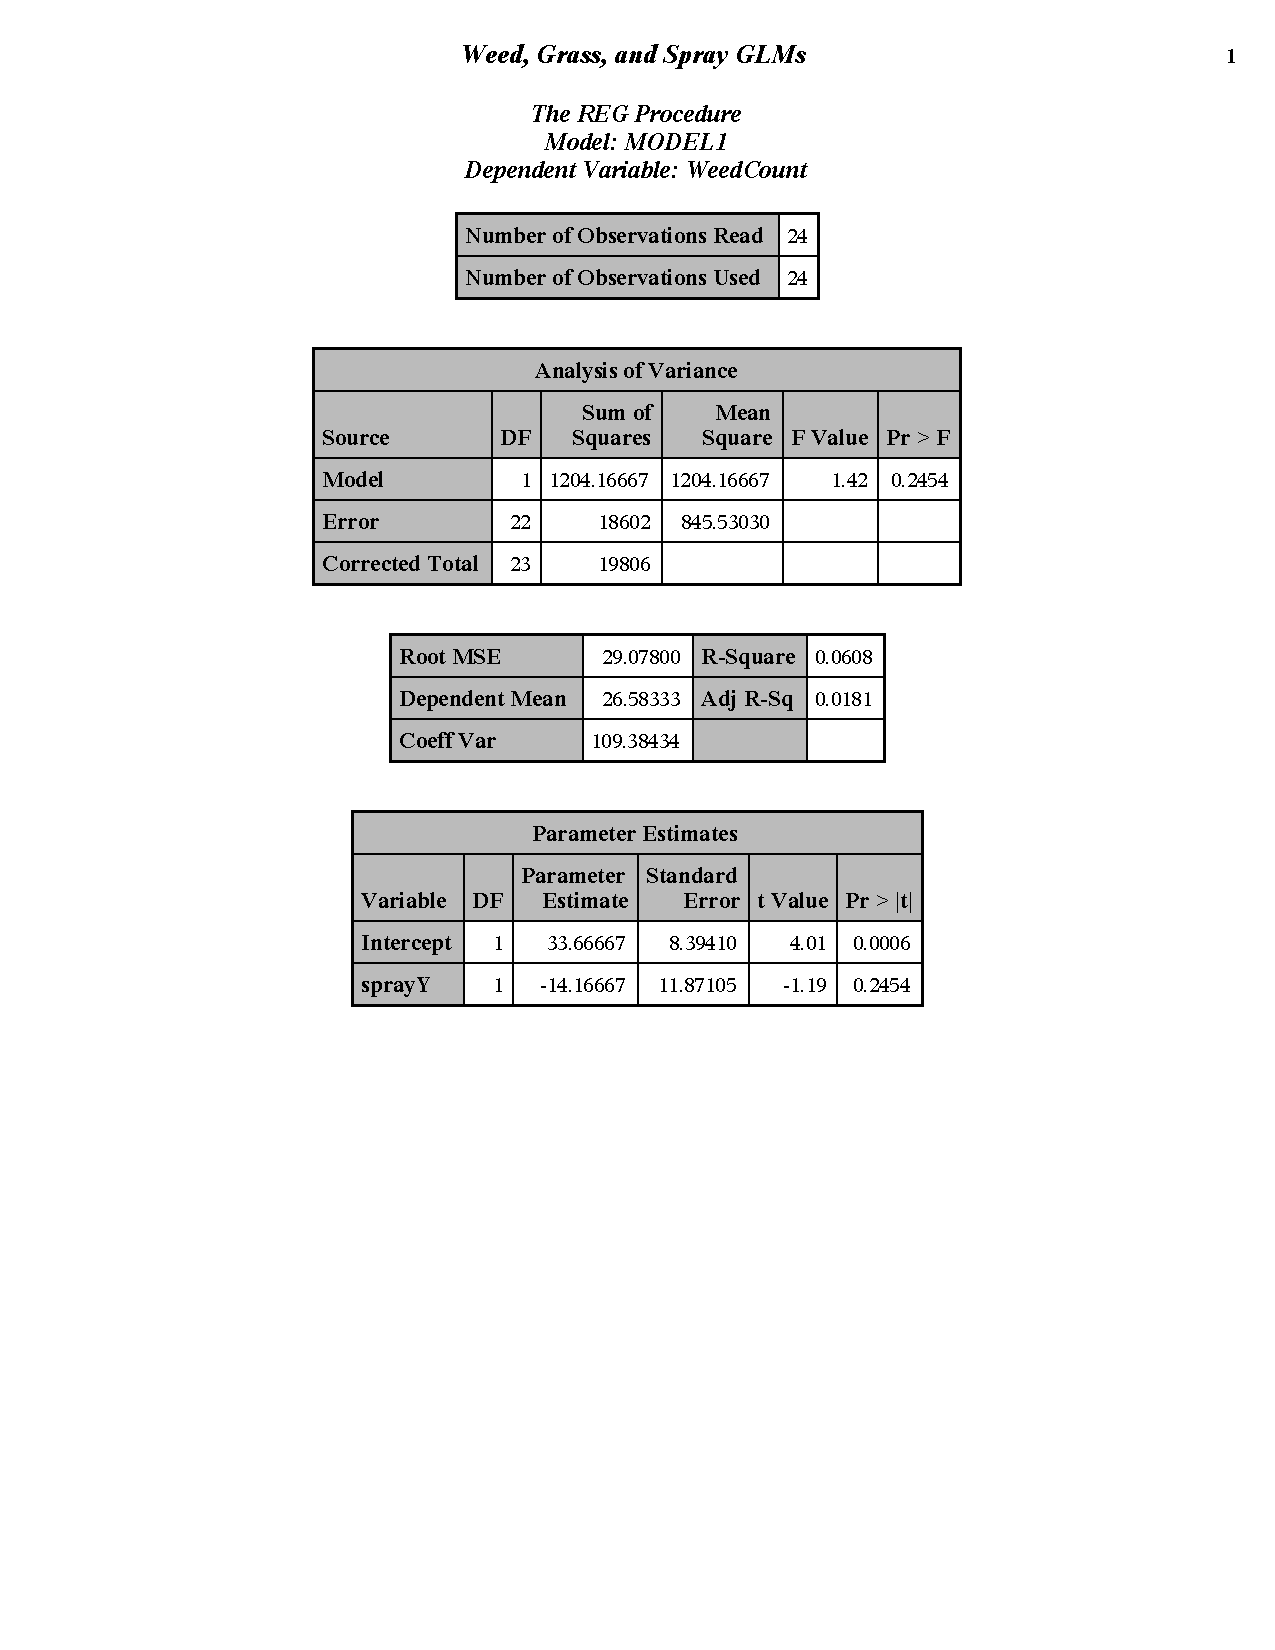
\includegraphics{WeedsandGrass}



%\newpage
%Exercises:
%\begin{enumerate}
%\item Hiking data: test for lack-of-fit of quadratic model 
%%, based on
%($df=2,15$).  Also, let $x'=\log_e(x+1)$.  Obtain a plot 
%of $y \mbox{ vs }x'$.  Test for lack-of-fit of a model in which 
%mean plant height is linear in $x'$.
%%\item Test for lack-of-fit of SLR models in Rao exercises 10.1,10.2
%\item Test for lack-of-fit of of SLR model for corn yields and rainfall
%data.  Test for lack-of-fit of quadratic model for same data.  Specify
%$SS[\mbox{lack-of-fit}]$ and $SS[\mbox{pure error}]$. 
%\end{enumerate}
%  %\newpage
%  %%\pagestyle{myheadings}
%  %%\markright{Orthogonal polynomial contrasts}
%  %%\setlength{\topmargin}{0pt}
%  %%\setlength{\oddsidemargin}{0pt}
%  %%\large
%  %%\begin{LARGE}
%  %\noindent
%  %%{\bf ST 512: Exptl Stats for Biol. Sciences II - Fall, 2003}\\
%  %\cu{Orthogonal polynomial contrasts} 
%  %%{\bf Problems } Ch. 9,13
%  %\bigkn
%  %%\begin{center}
%  %%\epsfig{file=psfiles/powerfinal.ps,height=3in,width=3in,angle=270} 
%  %%\end{center}
%  %\noindent
%  %Example: poultry science experiment measures bodyweights of chickens
%  %from $a=4$ diet groups, characterized by protein concentration in
%  %diet.
%  %\begin{itemize}
%  %\item $Y$: 21-day bodyweights of chickens 
%  %\item completely randomized design with one factor, protein in diet, 
%  %with four {\em equally spaced} levels.
%  %\item thanks to P. Plumstead for data.
%  %%The design is balanced, with $n$ pens (of chickens) in 
%  %%each treatment group.  
%  %\item $n=18$ pens, $N=72$. 
%  %\end{itemize}
%  %%(Let $y_{ij}$ denote 
%  %%bodyweight in $j^{th}$ pen assigned $i^{th}$ treatment group.) 
%  %\begin{center}
%  %\begin{tabular}{c|c|c|c|c}
%  %diet   & $x$: level of & diet mean & diet std. dev. & Tukey \\
%  %group & protein & $\bar{y}_{i+}$ & $s_i$ & grouping \\ \hline
%  %                                                                                
%  %1 &              21.8         & 993        & 38\\
%  %2 &              23.5         & 1003 & 28\\
%  %3 &              25.2         & 1022 & 39\\
%  %4 &              26.9         & 1050 & 32\\ 
%  %\hline
%  %\end{tabular}
%  %\end{center}
%  %One-way ANOVA table
%  %\end{LARGE}
%  %\begin{verbatim}
%  %                               Sum of
%  % Source             DF        Squares   Mean Square  F Value  Pr > F
%  % Model               3     34311.7666    11437.2555     9.57  <.0001
%  % Error               68    81279.4678     1195.2863                 
%  % Corrected Total     71   115591.2344                               
%  %
%  %R-Square     Coeff Var      Root MSE    AMBW21D Mean
%  %0.296837      3.399254      34.57291        1017.073
%  %\end{verbatim}
%  %\begin{LARGE}
%  %\newpage
%  %Some omitted exam questions:
%  %\begin{enumerate}
%  %\item Sketch a plot of mean bodyweight at 21 days against protein
%  %content.
%  %%\vspace{2in}
%  %\item
%  %Consider the following three sample contrasts
%  %\begin{eqnarray*}
%  %\hat\theta_1 & = & -3 \tmean{1} - \ \tmean{2} + \ \tmean{3} + 3 \tmean{4} \\
%  %\hat\theta_2 & = & \ \ \ \ \tmean{1} - \ \tmean{2} - \ \tmean{3} + \ \tmean{4} \\
%  %\hat\theta_3 & = & \ \ -\tmean{1} + 3 \tmean{2} -3 \tmean{3} + \ \tmean{4} 
%  %\end{eqnarray*}
%  %\begin{enumerate}
%  %\item True/false: These estimated contrasts are orthogonal.
%  %\item True/false: If contrast sums of squares are obtained, then
%  %$$SS[\hat\theta_1] + SS[\hat\theta_2] + SS[\hat\theta_3]  = SS[Trt]?$$
%  %\item Report $\hat\theta_1,\hat\theta_2,\hat\theta_3$.
%  %\item Provide an expression for the standard error of $\hat\theta_2$. 
%  %\item Estimate the standard error of $\hat\theta_2$.
%  %\item Report $SS(\hat\theta_1)$.
%  %\end{enumerate}
%  %\item Fitting the SLR model leads to $SS[Reg]=32742$ and $SS[Tot]=115591$.
%  %\begin{enumerate}
%  %\item Report the $F$-ratio for testing for a lack-of-fit of the linear model.
%  %\item
%  %The appropriate critical value for a test with level $\alpha=0.05$ is
%  %$F^{*}=3.13$.  
%  %Draw a conclusion about the adequacy of the linear model
%  %using $\alpha=0.05$: is there evidence that the linear model is inadequate?
%  %%%\end{enumerate}
%  %\end{enumerate}
%  %\end{enumerate}
%  %\newpage 
%  %\noindent
%  %The contrasts in problem 2 are called {\em orthogonal polynomial contrasts}.
%  %%For example, the contrast $\hat\theta_2$ can be used to test for a quadratic
%  %%association between weight $y$ and protein content $x$.  
%  %The table below gives coefficients for orthogonal polynomial contrasts 
%  %for balanced single-factor experiments with 3, 4, or 5 equally spaced 
%  %levels.
%  %\begin{center}
%  %\begin{tabular}{ccc|ccccc|c}
%  %Factor& Poly.& & \multicolumn{5}{c|}{Coefficients for} & \\
%  %levels & Degree & contrast & $\bar{y}_{1+}$ & $\bar{y}_{2+}$ & $\bar{y}_{3+}$ & $\bar{y}_{4+}$ & $\bar{y}_{5+}$ & $SS(\hat\theta_i)$\\ \hline
%  %3 & 1 &$\hat\theta_1$& -1 & 0 & 1 & & & $R(\beta_1|\beta_0)$\\
%  %  & 2 &$\hat\theta_2$& 1 & -2 & 1 & & & $R(\beta_2|\beta_0,\beta_1)$\\ \hline
%  %4 & 1 &$\hat\theta_1$& -3 & -1 & 1 & 3 & & $R(\beta_1|\beta_0)$\\
%  %  & 2 &$\hat\theta_2$& 1 & -1 & -1 & 1 & & $R(\beta_2|\beta_0,\beta_1)$\\ 
%  %  & 3 &$\hat\theta_3$& -1 & 3 & -3 & 1 & & $R(\beta_3|\beta_0,\beta_1,\beta_2)$\\  \hline
%  %5 & 1 &$\hat\theta_1$& -2 & -1 & 0 & 1 & 2 & ?\\
%  %  & 2 &$\hat\theta_2$& 2 & -1 & -2 & -1 & 2 & ?\\
%  %  & 3 &$\hat\theta_3$& -1 & 2 & 0 & -2 & 1 & ?\\
%  %  & 4 &$\hat\theta_4$& 1 & -4 & 6 & -4 & 1 & ?\\ \hline
%  %\end{tabular}
%  %\end{center}
%  %Rightmost column indicates extra SS in MLR of the form
%  %$$\mu(x) = \beta_0 + \beta_1 x + \beta_2 x^2 + \cdots.$$
%  %The contrast corresponding to a polynomial of degree $p$
%  %can be used to test for a $p^{th}$ degree association:
%  %
%  %\noindent
%  %%For Plumstead's data, 
%  %\begin{itemize}
%  %\item large $|\hat\theta_1|$ indicates
%  %linear association between $y$ and $x$.
%  %\item large $|\hat\theta_2|$ indicates
%  %quadratic association between $y$ and $x$.
%  %\item large $|\hat\theta_3|$ indicates 
%  %cubic association between $y$ and $x$.
%  %\end{itemize}
%  %This is computationally (and otherwise) easier than
%  %fitting polynomial regressions of various degrees.
%  %\end{LARGE}
%  %
%  %\newpage
%  %%For Plumstead's data, we could code them this way:
%  %\begin{verbatim}
%  %Proc GLM; 
%  %   title "protein concentration and chicken weights"; 
%  %   class cp;
%  %   MODEL AMBW21D=cp;
%  %   contrast 'cp linear' cp -3 -1 1 3;
%  %   contrast 'CP quadratic' CP 1 -1 -1 1;
%  %   contrast 'CP cubic' CP -1 3 -3 1; 
%  %   contrast 'all three' CP -3 -1 1 3, 
%  %                        cp 1 -1 -1 1, 
%  %                        cp -1 3 -3 1; 
%  %   /* 'all three' tests that the 3-vector of contrasts is (0,0,0)' */
%  %   estimate 'cp linear' cp -3 -1 1 3;
%  %   estimate 'CP quadratic' CP 1 -1 -1 1;
%  %   estimate 'CP cubic' CP -1 3 -3 1; 
%  %RUN;
%  %proc glm; /* no class statement will fit regression model*/
%  %   model ambw21d=cp cp*cp cp*cp*cp; 
%  %run;
%  %proc glm; 
%  %   model ambw21d=cp; 
%  %run;
%  %                 protein concentration and chicken weights                1
%  %                             The GLM Procedure
%  % 
%  %               Class         Levels    Values
%  %               CP                 4    21.8 23.5 25.2 26.9 
%  % 
%  %                                     Sum of
%  % Source                    DF       Squares   Mean Square  F Value  Pr > F
%  % Model                      3    34311.7666    11437.2555     9.57  <.0001
%  % Error                     68    81279.4678     1195.2863                 
%  % Corrected Total           71   115591.2344                               
%  %
%  % Contrast                  DF   Contrast SS   Mean Square  F Value  Pr > F
%  % cp linear                  1   32741.55648   32741.55648    27.39  <.0001
%  % CP quadratic               1    1568.66674    1568.66674     1.31  0.2560
%  % CP cubic                   1       1.54337       1.54337     0.00  0.9714
%  % all three                  3   34311.76658   11437.25553     9.57  <.0001
%  %
%  %                                            Standard
%  %Parameter                   Estimate           Error    t Value    Pr > |t|
%  %cp linear                 190.734127      36.4430498       5.23      <.0001
%  %CP quadratic               18.670635      16.2978273       1.15      0.2560
%  %CP cubic                    1.309524      36.4430498       0.04      0.9714
%  %\end{verbatim}
%  %\newpage
%  %\begin{verbatim}
%  %                 protein concentration and chicken weights                3
%  %
%  %                             The GLM Procedure
%  %
%  %                                     Sum of
%  % Source                    DF       Squares   Mean Square  F Value  Pr > F
%  % Model                      3    34311.7666    11437.2555     9.57  <.0001
%  % Error                     68    81279.4678     1195.2863                 
%  % Corrected Total           71   115591.2344                               
%  %
%  % Source                    DF     Type I SS   Mean Square  F Value  Pr > F
%  % CP                         1   32741.55648   32741.55648    27.39  <.0001
%  % CP*CP                      1    1568.66674    1568.66674     1.31  0.2560
%  % CP*CP*CP                   1       1.54337       1.54337     0.00  0.9714
%  %
%  %                                       Standard
%  %     Parameter         Estimate           Error    t Value    Pr > |t|
%  %     Intercept      1060.706771     17690.23708       0.06      0.9524
%  %     CP               11.320308      2192.80559       0.01      0.9959
%  %     CP*CP            -1.630049        90.32122      -0.02      0.9857
%  %     CP*CP*CP          0.044424         1.23628       0.04      0.9714
%  %
%  %                 protein concentration and chicken weights                6
%  %
%  %                             The GLM Procedure
%  % 
%  %                                     Sum of
%  % Source                    DF       Squares   Mean Square  F Value  Pr > F
%  % Model                      1    32741.5565    32741.5565    27.66  <.0001
%  % Error                     70    82849.6779     1183.5668                 
%  % Corrected Total           71   115591.2344                               
%  %
%  %                                       Standard
%  %     Parameter         Estimate           Error    t Value    Pr > |t|
%  %     Intercept      743.8748249     52.10077470      14.28      <.0001
%  %     CP              11.2196545      2.13317368       5.26      <.0001
%  %\end{verbatim}
%  %\begin{LARGE}
%  %Note MSE.  Linear regression on $x$ preferred to one-factor
%  %model for Plumstead's data.  Multiple comparisons among treatment means 
%  %might be unnecessary.
%  %%
%  %%\vspace{2in} 
%  %%






%\end{LARGE}
%\end{document}





























\newpage
%{\bf ST 512: Exptl Stats for Biol. Sciences II - Fall, 2003}\\
%Dr. Jason A. Osborne\\
%{\bf Supplement on design imbalance}
\noindent
{\bf Topic:} Supplement on design imbalance \\
{\bf Reading:} None \\
%{\bf Problems } Ch. 9,13
\bigkn
%\begin{center}
%\epsfig{file=psfiles/powerfinal.ps,height=3in,width=3in,angle=270} 
%\end{center}
\noindent
Recall the $2\times 2$ cholesterol study.  Suppose the study is
unbalanced and the data are given by
\begin{center}
\begin{tabular}{|c|cc|c|} \hline
& \multicolumn{2}{c}{Gender} & \\
Age & Male & Female & Marginal mean \\ \hline
young & 271,192,189,209, & 162 & $\bar{y}_{1++}=212.3$ \\ 
& 227,236 & & \\  \hline
old & 289 & 262,193,224,201 & $\bar{y}_{2++}=221.6$ \\
& & 161,178,265 & \\  \hline
& $\bar{y}_{+1+}=230.4$ & $\bar{y}_{+2+}=205.8$ & \\ \hline
\end{tabular}
\end{center}
$$\bar{y}_{11}=220.7,\ \bar{y}_{12}=162, \ \bar{y}_{21}=289,\ \bar{y}_{22}=212.$$
%(Level 1 of age (A) is young and level 1 of gender (B) is male.) \\
%\par
\noindent
Consider an additive two-factor ANOVA model:
$$Y_{ijk} = \mu + \alpha_i + \beta_j + E_{ijk}$$ 
%M_2: Y_{ijk} &=& \mu + \alpha_i + \beta_j + (\alpha\beta)_{ij} + E_{ijk}.
Exercise: finish parametric expressions for expected values below:
\begin{eqnarray*}
E(\bar{Y}_{1++}) & = & \mu + \alpha_1 + \frac{1}{7}\left(6 \beta_1 + \beta_2\right) \\
E(\bar{Y}_{2++}) & = & \mu + \alpha_2 + \frac{1}{8}\left(\beta_1 + 7\beta_2\right) \\
E(\bar{Y}_{+1+}) & = & \\ % \mu + \frac{1}{7}\left(6 \alpha_1 + \alpha_2\right) + \beta_1\\
E(\bar{Y}_{+2+}) & = & %\mu + \frac{1}{8}\left(\alpha_1 + 7\alpha_2\right)+ \beta_2 
\end{eqnarray*}
Marginal sample means are not real useful in this unbalanced study.
\\
%\par\noindent
Q: How are group population means estimated then?
\\
%\par\noindent
A: {\em Least squares means} (what would be estimated by marginal means
if design {\em were} 
balanced).  
\newpage
\noindent
Parametric expressions for all the population means of interest
are given below for the additive model:
\begin{center}
\begin{tabular}{c|c|c}
Population group & effect of interest& estimate \\ \hline
Young folks & $\mu + \alpha_1 + \frac{1}{2}(\beta_1 + \beta_2)$ &  188.03\\
Older folks & $\mu + \alpha_2 + \frac{1}{2}(\beta_1 + \beta_2)$ &  \\
Men & $\mu + \frac{1}{2}(\alpha_1 + \alpha_2) + \beta_1$ &  \\
Women & $\mu + \frac{1}{2}(\alpha_1 + \alpha_2) + \beta_2$ &  \\
Young men & $\mu + \alpha_1 + \beta_1$ & \\
Older men & $\mu + \alpha_2 + \beta_1$ & \\
Young women & $\mu + \alpha_1 + \beta_2$ & \\
Older women & $\mu + \alpha_2 + \beta_2$ & \\ \hline
\end{tabular}
\end{center}
\noindent
Invoking the command {\tt lsmeans age gender;} will report
least squares estimates for the first four means above.
\begin{large}
\begin{verbatim}
                             The GLM Procedure
                            Least Squares Means

                                          Standard
            gender        y LSMEAN           Error    Pr > |t|
            m           251.525773       16.233482      <.0001
            w           183.597938       15.842256      <.0001

                                         Standard
              age        y LSMEAN           Error    Pr > |t|
              jr       188.025773       16.233482      <.0001
              sr       247.097938       15.842256      <.0001
\end{verbatim}
\end{large}
All of these quantities are estimated using linear combinations of the
treatment means of the form:
$$ \hat\theta = c_{11}\bar{y}_{11+} + c_{12}\bar{y}_{12+}  + c_{21}\bar{y}_{21+}  + c_{22}\bar{y}_{22+}.$$ 
The coefficients are chosen so that $E(\hat\theta)=\theta$ 
and $\sum \frac{c_{ij}^2}{n_{ij}}$ is minimized.
\newpage
\noindent
Example: What are the coefficients for the contrast which estimates
the population mean for young folks, $\mu+\alpha_1 + \frac{1}{2}(\beta_1 + \beta_2)$ with minimum variance?
\begin{eqnarray*}
c_{11} + c_{12} &=& 1 (\mbox{coeff for }\alpha_1)\\
c_{21} + c_{22} &=& 0 (\mbox{coeff for }\alpha_2)\\
c_{11} + c_{21} &=& \frac{1}{2} (\mbox{coeff for }\beta_1) \\
c_{12} + c_{22} &=& \frac{1}{2} (\mbox{coeff for }\beta_2) 
\end{eqnarray*}
Variance is then proportional to
$$ \frac{c_{11}^2}{n_{11}} + \frac{c_{12}^2}{n_{12}} + \frac{c_{21}^2}{n_{21}} + \frac{c_{22}^2}{n_{22}} = \frac{c_{11}^2}{n_{11}} + \frac{(1-c_{11})^2}{n_{12}} + \frac{(\frac{1}{2}-c_{11})^2}{n_{21}} + \frac{(c_{11}-\frac{1}{2})^2}{n_{22}}$$ 
which is minimized at $c_{11}=\frac{66}{97}$ by setting the derivative to zero
and solving.  The least squares mean is then
$$ \hat\theta = \frac{66}{97}\bar{y}_{11+} + (1-\frac{66}{97}) \bar{y}_{12+}  
+(\frac{1}{2}-\frac{66}{97}) \bar{y}_{21+}  +(\frac{66}{97} - \frac{1}{2})\bar{y}_{22+} = 188.03.$$ 
%\\
%\par\noindent
Similarly for old folks, the contrast with minimum variance has
$$c_{11}=18/97=-c_{12}$$ 
and 
$$c_{21}=\frac{1}{2}-18/97,c_{22}=\frac{1}{2}+18/97$$
so that the estimate for the old folks mean is
$$ \frac{18}{97}\bar{y}_{11+} - \frac{18}{97} \bar{y}_{12+}  
+(\frac{1}{2}-\frac{18}{97}) \bar{y}_{21+}  +(\frac{1}{2}+\frac{18}{97} )\bar{y}_{22+} = 247.1.$$
Exercise: obtain least squares estimators and estimates of marginal 
means for men and women as well as for each age$\times$gender combination.
\newpage
\noindent
Q: Is there an age effect?  Should we base our conclusion on 
$$ \sum_i\sum_j\sum_k (\bar{y}_{i++} - \bar{y}_{+++})^2 = 325.6?$$
A: Might not be a good idea if factor B has an effect. \\
(This is the type I SS for Age if Age is the first factor entered 
into the model, or the so-called unadjusted sum of squares for age.) \\
%A: Better to use type II sums of squares, which adjusts for other
%factors not involving $A$. \\
\par\noindent
Alternatively, consider the contrast 
%$$ \hat\theta_{age} = \hat\alpha_1 - \hat\alpha_2.$$
$$ \theta_{age} = \alpha_1 - \alpha_2.$$
We can obtain the coefficients of the LS estimate of this contrast
and then use them to get $SS[\hat\theta_{age}]$, which is the sum
of squares for the age effect adjusted for gender, or type II sum
of squares for age:
$$ \hat\theta_{age} = \hat\alpha_1 - \hat\alpha_2 = 
 c_{11}\bar{y}_{11+} + c_{12}\bar{y}_{12+}  + c_{21}\bar{y}_{21+}  + c_{22}\bar{y}_{22+}$$ 
where 
\begin{eqnarray*}
c_{11} + c_{12} & = & 1 (\mbox{coeff for }\alpha_1)\\
c_{21}+c_{22} & = & -1 (\mbox{coeff for }\alpha_2) \\
c_{11}+c_{21} & = & 0  (\mbox{coeff for }\beta_1)\\
c_{12}+c_{22} & = & 0 (\mbox{coeff for }\beta_2)
\end{eqnarray*}
$\Var(\hat\theta_{age})$ is minimized when $c_{11}=\frac{48}{97}$
which leads to 
$$\hat\theta_{age}=-59.07$$
with
%\begin{eqnarray*}
%$$
%SS[\hat\theta_{age}] = \frac{(-59.1)^2}{\frac{(\frac{48}{97})^2}{6} + \frac{(-1-\frac{48}{97})^2}{6}  + \frac{(\frac{-48}{97})^2}{6} + \frac{(-1+\frac{48}{97})^2}{6}} = 6044.$$ 
$$
SS[\hat\theta_{age}] = \frac{(-59.07)^2}{\frac{(\frac{48}{97})^2}{6} + \frac{(-1-\frac{48}{97})^2}{1}  + \frac{(\frac{-48}{97})^2}{1} + \frac{(-1+\frac{48}{97})^2}{7}} = 6044.$$ 
%(Thanks to Carl DiCasoli for fixing this.)
%& = & 6044.
%\end{eqnarray*}
\newpage
\begin{large}
\begin{verbatim}
/*
I   221  213  202  183  185  197  162
II  271  192  189  209  227  236  142
III 262  193  224  201  161  178  265
IV  192  253  248  278  232  267  289
*/
options ls=75;
data one;
   input gender $ age $2. @;
   do i=1 to 7;
      input y @@;
      output;
   end;
cards;
w jr  .  .  .  .  .  .  162 
m jr  271  192  189  209  227  236  .
w sr  262  193  224  201  161  178  265
m sr  .  .  .  .  .  .  289
;
run;

proc glm;
   class age gender; 
   model y=age gender/solution; 
   lsmeans gender age/stderr; 
   estimate "lsmean for young folks" intercept 2 age 2 0 gender 1 1/divisor=2; 
   estimate "lsmean for older folks" intercept 2 age 0 2 gender 1 1/divisor=2; 
   estimate "lsmean for men" intercept 2 age 1 1 gender 2 0/divisor=2; 
   estimate "lsmean for women" intercept 2 age 1 1 gender 0 2/divisor=2; 
   estimate "lsmean for young men" intercept 1 age 1 0 gender 1 0;
   estimate "lsmean for young women" intercept 1 age 1 0 gender 0 1;
   estimate "lsmean for old men" intercept 1 age 0 1 gender 1 0;
   estimate "lsmean for old women" intercept 1 age 0 1 gender 0 1;
   contrast "age effect" age 1 -1;
   estimate "age effect" age 1 -1;
   contrast "gender effect" gender 1 -1;
   means gender age; 
run;

\end{verbatim}
\newpage
\begin{verbatim}

                              The SAS System                              1
                             The GLM Procedure
                         Class Level Information
 
                      Class         Levels    Values
                      age                2    jr sr 
                      gender             2    m w   

                       Number of observations    28

NOTE: Due to missing values, only 15 observations can be used in this 
      analysis.

                                     Sum of
 Source                    DF       Squares   Mean Square  F Value  Pr > F
 Model                      2    8318.06735    4159.03368     3.42  0.0669
 Error                     12   14606.86598    1217.23883                 
 Corrected Total           14   22924.93333                               

            R-Square     Coeff Var      Root MSE        y Mean
            0.362839      16.05812      34.88895      217.2667

 Source                    DF     Type I SS   Mean Square  F Value  Pr > F
 age                        1    325.629762    325.629762     0.27  0.6144
 gender                     1   7992.437592   7992.437592     6.57  0.0249

 Source                    DF   Type III SS   Mean Square  F Value  Pr > F
 age                        1   6044.348306   6044.348306     4.97  0.0457
 gender                     1   7992.437592   7992.437592     6.57  0.0249

                                         Standard
  Parameter            Estimate             Error    t Value    Pr > |t|
  Intercept         213.1340206 B     12.77243521      16.69      <.0001
  age       jr      -59.0721649 B     26.50916484      -2.23      0.0457
  age       sr        0.0000000 B       .                .         .    
  gender    m        67.9278351 B     26.50916484       2.56      0.0249
  gender    w         0.0000000 B       .                .         .    
\end{verbatim}
\newpage
\begin{verbatim}
                            Least Squares Means

                                          Standard
            gender        y LSMEAN           Error    Pr > |t|
            m           251.525773       16.233482      <.0001
            w           183.597938       15.842256      <.0001

                                         Standard
              age        y LSMEAN           Error    Pr > |t|
              jr       188.025773       16.233482      <.0001
              sr       247.097938       15.842256      <.0001
 
 Contrast                  DF   Contrast SS   Mean Square  F Value  Pr > F
 age effect                 1   6044.348306   6044.348306     4.97  0.0457
 gender effect              1   7992.437592   7992.437592     6.57  0.0249

                                             Standard
 Parameter                    Estimate          Error   t Value   Pr > |t|
 lsmean for young folks     188.025773     16.2334818     11.58     <.0001
 lsmean for older folks     247.097938     15.8422561     15.60     <.0001
 lsmean for men             251.525773     16.2334818     15.49     <.0001
 lsmean for women           183.597938     15.8422561     11.59     <.0001
 lsmean for young men       221.989691     13.7197962     16.18     <.0001
 lsmean for young women     154.061856     26.2714097      5.86     <.0001
 lsmean for old men         281.061856     26.2714097     10.70     <.0001
 lsmean for old women       213.134021     12.7724352     16.69     <.0001
 age effect                 -59.072165     26.5091648     -2.23     0.0457
\end{verbatim}
\end{large}

\vspace{1in}

\noindent
(These notes were adapted from one of Dr. Dickey's lectures:) \\
\begin{large}
\href{http://www.stat.ncsu.edu/people/dickey/courses/st512/crsnotes/rnotes_unbal.htm}
{http://www.stat.ncsu.edu/people/dickey/courses/st512/crsnotes/rnotes\_unbal.htm}
\end{large}


%\begin{large}
%%%{\tt http://www.stat.ncsu.edu/$\tilde{}$st512\_info/dickey/crsnotes/rnotes\_unbal.htm}
%\begin{verbatim}
%http://www.stat.ncsu.edu/~st512_info/dickey/crsnotes/rnotes_unbal.htm
%\end{verbatim}
%\end{large}

\newpage
























\newpage
\cu{Analysis of variance in nested designs}
Consider a two-factor design in which factor $B$ is nested in factor $A$.
Let $Y_{ijk}$ denote the $k^{th}$ response at level $j$ of factor $B$
within level $i$ of factor $A$.  A model: \\
\begin{center}
\fbox{$Y_{ijk} = \mu + \alpha_i + \beta_{j(i)} + E_{ijk}$}
\end{center}
for $i=1,2,\ldots,a,\ j=1,2,\ldots,b_i, \ k=1,2,\ldots,n$
\bigkn
$SS[Tot]$ can be broken down into components reflecting variability 
due to $A$, $B(A)$ and variability not due to either factor ($SS[E]$):
$SS[Tot]=SS[A]+SS[B(A)]+SS[E]$ %(compare w/ p. 639.)  
\begin{eqnarray*}
SS[Tot] & = &\sum_i \sum_j \sum_k (y_{ijk}-\gmeanb)^2 \\
%SS[A] & = &\sum_i \sum_j \sum_k (y_{i++}-\gmeanb)^2 \\
SS[A] & = &\sum_i \sum_j \sum_k (\tmean{i+}-\gmeanb)^2 \\
SS[B(A)] & = &\sum_i \sum_j \sum_k (\tmean{ij}-\tmean{i+})^2 \\
SS[E] & = & \sum_i \sum_j \sum_k (y_{ijk}-\tmean{ij})^2 
% & = & SS[Tot]-SS[A]-SS[B(A)] 
\end{eqnarray*}
The ANOVA table looks like 
\bigkn
\begin{tabular}{|c|c|c|c|c|} \hline
& & Sum of & Mean & \\
Source & d.f. & squares & Square & F \\ \hline
$A$ & $a-1$ & $SS[A]$ & $MS[A]=\frac{SS[T]}{(a-1)}$ & $F_A=\frac{MS[A]}{MS[E]}$ \\ 
$B(A)$ & $\sum_i (b_i-1)$ & $SS[B(A)]$ & $MS[B(A)]=\frac{SS[B(A)]}{\sum(b_i-1)}$ & $F_{B(A)}=\frac{MS[B(A)]}{MS[E]}$ \\ 
%Error & $df_E=N-1$ & $SS[E]$ & $MS[E]=\frac{SS[E]}{(N-t)}$ & \\
Error & $N-\sum b_i$ & $SS[E]$ & $MS[E]=\frac{SS[E]}{(N-t)}$ & \\
Total & $N-1$ & $SS[TOT]$ & &\\ \hline
\multicolumn{5}{c}{If $b_1 = b_2 = \cdots b_a=b$ then 
$\sum (b_i-1) = a(b-1) \mbox{ and }df_E=ab(n-1).$}
\end{tabular}
\noindent
%If %the same number of 
%$b_1 = b_2 = \cdots b_a=b$ then 
%$$\sum (b_i-1) = a(b-1) \mbox{ and }df_E=ab(n-1).$$
\newpage
\cu{Inference from nested designs}
\bigkn
To test $H_0: \alpha_i \equiv 0$, use $F_A$ on $a-1$ and $df_E$ degrees
of freedom. 
\bigkn
To test $H_0: \beta_{j(i)} \equiv 0$, for all $i,j$, use $F_{B(A)}$ 
on $\sum(b_i-1)$ and $df_E$ degrees of freedom.
\bigkn
For the diabetics blood sugar data, with $\gmeanb=22.3$ and
means
\begin{center}
\begin{tabular}{|llccc|} \hline
Drug & Type of & Mean & Variance & Mean \\
($i$) & Administration $(j)$ & $\bar{y}_{j(i)}$ & $s_{j(i)}^2$ & $\bar{y}_{+(i)}$\\ \hline
Brand I tablet & $30 mg \times 1$ & 15.7 & 6.3 & 17.7\\
& $15 mg \times 2$ & 19.7 & 9.3 & \\
Brand II tablet & $20 mg \times 1$ & 20 & 1 & 18.7 \\
& $10 mg \times 2$ & 17.3 & 6.3 & \\
Insulin injection & $$ before breakfast  & 28  & 4 & 30.5\\
& before supper & 33 & 9 & \\ \hline
\end{tabular}
\end{center}
%(Grand mean is $\bar{y}_{+(+)}=22.3$.)
\begin{eqnarray*}
SS[A] &=& 2(3) [(17.7-22.3)^2 + (18.7-22.3)^2 + (30.5 - 22.3)^2 \\
      &=& 611.4 \\ 
SS[B(A)] &=& 3 [(15.7-17.7)^2 + (19.7-17.7)^2 + (20.0 - 18.7)^2 \\
%&+& (17.3-18.7)^2 + (28-30.5)^2 + (33 - 30.5)^2] \\
&& + (17.3-18.7)^2 + (28-30.5)^2 + (33 - 30.5)^2] \\
&=&  72.2 \\
SS[E] &=& 72
\end{eqnarray*}
Q1: How many $df$ associated with $SS[A]$? \\
Q2: How many $df$ associated with $SS[B(A)]$? \\
Q3: How many $df$ associated with $SS[E]$? \\
\newpage
\begin{large}
\begin{verbatim}
data one;
   infile "blsugar.dat" firstobs=2 dlm='09'x;
   input a b rep y;
   drug=a;  admin=b;
run;

proc glm;
   class a b;
   model y=a b(a);
   output out=two p=p r=r;
   means a b(a)/lsd;
   estimate "effect of B within A=1" b(a) -1 1; 
   estimate "effect of B within A=2" b(a) 0 0 -1 1; 
   estimate "effect of B within A=3" b(a) 0 0 0 0 -1 1; 
   estimate "A=1 mean - A=2 mean" a 1 -1; 
   estimate "A=1 mean - A=3 mean" a 1 0 -1; 
   estimate "A=2 mean - A=3 mean" a 0 1 -1; 
run;

                             The GLM Procedure

                                     Sum of
 Source                    DF       Squares   Mean Square  F Value  Pr > F
 Model                      5   683.6111111   136.7222222    22.79  <.0001
 Error                     12    72.0000000     6.0000000                 
 Corrected Total           17   755.6111111                               

            R-Square     Coeff Var      Root MSE        y Mean
            0.904713      10.99522      2.449490      22.27778

 Source                    DF     Type I SS   Mean Square  F Value  Pr > F
 a                          2   611.4444444   305.7222222    50.95  <.0001
 b(a)                       3    72.1666667    24.0555556     4.01  0.0344

                                             Standard
 Parameter                    Estimate          Error   t Value   Pr > |t|

 effect of B within A=1      4.0000000     2.00000000      2.00     0.0687
 effect of B within A=2     -2.6666667     2.00000000     -1.33     0.2072
 effect of B within A=3      5.0000000     2.00000000      2.50     0.0279
 A=1 mean - A=2 mean        -1.0000000     1.41421356     -0.71     0.4930
 A=1 mean - A=3 mean       -12.8333333     1.41421356     -9.07     <.0001
 A=2 mean - A=3 mean       -11.8333333     1.41421356     -8.37     <.0001
\end{verbatim}
\end{large}

%%\begin{large}
%%\begin{verbatim}
%%             a            N       Mean          
%%
%%             1            6       17.7       
%%             2            6       18.7      
%%             3            6       30.5
%%
%%       Level of     Level of           --------------y--------------
%%       b            a            N             Mean          Std Dev
%%
%%       1            1            3       15.6666667       2.51661148
%%       2            1            3       19.6666667       3.05505046
%%       1            2            3       20.0000000       1.00000000
%%       2            2            3       17.3333333       2.51661148
%%       1            3            3       28.0000000       2.00000000
%%       2            3            3       33.0000000       3.00000000
%%\end{verbatim}
%%\end{large}
\newpage
Conclusions?
\begin{itemize}
\item The administration effect $B$ (nested in the type of drug 
effect $A$) is statistically significant $(p=0.0344)$.  This is 
due mostly to the before breakfast/supper difference, which is 
estimated to be 
%$$\widehat{(\alpha\beta_{2(3)})} - \widehat{(\alpha\beta_{1(3)})} =
%5 mg/dl$$
$$ \bar{y}_{32+} - \bar{y}_{31+} = 5 mg/dl$$
with an (estimated) standard error of $SE=2=?$.  
\item
The effect of type of drug (factor $A$) is highly significant
$(p<0.0001)$.  Unadjusted pairwise comparisons indicate that the insulin 
injections yield greater changes, on average, in blood sugar than either 
pill and the mean changes brought by the pills don't differ significantly.
\item The following contrasts may be of interest:
\begin{eqnarray*}
\theta_1 &=& \mu_{1(3)} - \frac{1}{4}(\mu_{1(1)}+\mu_{2(1)}+\mu_{1(2)}+\mu_{2(2)})\\
\theta_2 &=& \mu_{2(3)} - \frac{1}{4}(\mu_{1(1)}+\mu_{2(1)}+\mu_{1(2)}+\mu_{2(2)})
\end{eqnarray*}
Exercise: Estimate them and test their significance ($H_0: \theta_i=0$).
\end{itemize}
\bigkn
%Next packet of notes will analyze the last four datasets.
%These models are covered in Ch. 14.5 and 14.6.


























\newpage
\cu{Using nested factorial effects to get SAS to produce appropriate contrast sums}
\cu{of squares for factorial effects analysis of plant height and light source data}
\begin{small}
\begin{verbatim}
proc mixed method=type3;
   class pot treatment source intensity dark;
   model y=dark source(dark) intensity(dark) source*intensity(dark) dark ;
   random pot(source*intensity*dark);
   lsmeans dark source(dark) intensity(dark) source*intensity(dark);
run;
The SAS System                                                                                1
The Mixed Procedure

Class        Levels    Values
pot               2    1 2                           
treatment         5    AH AL BH BL DD                
source            3    A B D                         
intensity         3    D H L                         
dark              2    0 1                           
                                  Type 3 Analysis of Variance
 
                                    Sum of
Source                    DF       Squares   Mean Square  Expected Mean Square
dark                       1      4.493520      4.493520  Var(Residual) + 2                    
                                                          Var(pot(sour*inten*dark)) +          
                                                          Q(dark,source(dark),intensity        
                                                          (dark),source*intensi(dark))         
source(dark)               1     34.339600     34.339600  Var(Residual) + 2                    
                                                          Var(pot(sour*inten*dark)) +          
                                                          Q(source(dark),source*intensi(dark)) 
intensity(dark)            1      1.155625      1.155625  Var(Residual) + 2                    
                                                          Var(pot(sour*inten*dark)) +          
                                                          Q(intensity(dark),source*            
                                                          intensi(dark))                       
source*intensi(dark)       1      1.092025      1.092025  Var(Residual) + 2                    
                                                          Var(pot(sour*inten*dark))            
                                                          + Q(source*intensi(dark))            
pot(sour*inten*dark)       5      6.112350      1.222470  Var(Residual) + 2                    
                                                          Var(pot(sour*inten*dark))            
Residual                  10     10.264200      1.026420  Var(Residual)                        

                                                              Error
Source                Error Term                                 DF    F Value    Pr > F
dark                  MS(pot(sour*inten*dark))                    5       3.68    0.1133
source(dark)          MS(pot(sour*inten*dark))                    5      28.09    0.0032
intensity(dark)       MS(pot(sour*inten*dark))                    5       0.95    0.3756
source*intensi(dark)  MS(pot(sour*inten*dark))                    5       0.89    0.3880
pot(sour*inten*dark)  MS(Residual)                               10       1.19    0.3793
Residual              .                                           .        .       .    

 Covariance Parameter Estimates
 
Cov Parm                 Estimate
pot(sour*inten*dark)      0.09802
Residual                   1.0264
\end{verbatim}
\newpage
\begin{verbatim}
                                   Least Squares Means
 
                                                         Standard
Effect                source  intensity  dark  Estimate     Error    DF  t Value  Pr > |t|
dark                                     0      32.8350    0.2764     5   118.79    <.0001
dark                                     1      34.0200    0.5528     5    61.54    <.0001
source(dark)          A                  0      31.3700    0.3909     5    80.25    <.0001
source(dark)          B                  0      34.3000    0.3909     5    87.74    <.0001
source(dark)          D                  1      34.0200    0.5528     5    61.54    <.0001
intensity(dark)               H          0      32.5662    0.3909     5    83.31    <.0001
intensity(dark)               L          0      33.1038    0.3909     5    84.68    <.0001
intensity(dark)               D          1      34.0200    0.5528     5    61.54    <.0001
source*intensi(dark)  A       H          0      30.8400    0.5528     5    55.79    <.0001
source*intensi(dark)  A       L          0      31.9000    0.5528     5    57.70    <.0001
source*intensi(dark)  B       H          0      34.2925    0.5528     5    62.03    <.0001
source*intensi(dark)  B       L          0      34.3075    0.5528     5    62.06    <.0001
source*intensi(dark)  D       D          1      34.0200    0.5528     5    61.54    <.0001
\end{verbatim}
\end{small}
\cu{Inference for light effects}
Model for treatment combination ``$ijk$" and pot $l$, seedling $m$:
$$ Y_{ijklm} = \mu  + \delta_i + \alpha_{j(i)} + \beta_{k(i)} + (\alpha\beta)_{jk(i)} + P_{l(ijk)} + E_{ijklm}$$
For treatment effects, use $MS(Pot(treatments))$ as the error term.  \\
For example, for $H _0: \gamma_{jk}\equiv 0$ (intensity effect is constant across light types), use
$$ F=\frac{MS(\mbox{interaction(dark)})}{MS(\mbox{Pot(dark*source*intensity)})} = \frac{1.09}{1.22}=.89 (p=.3880)$$ 
Degrees of freedom: $(df=?,?)$ \\
Estimation of variance components:
$$\hat\sigma^2 = MS(E) = 1.02 (df=10)$$
$$\hat\sigma_{P(T)}^2 = \frac{MS(\mbox{pot(treatment)})-MS(E)}{2} = \frac{1.22-1.02}{2} = 0.098 (df=\widehat{df})$$
Correlation structure?  Intrapot correlation?
$$ \widehat{\mbox{Corr}} (Y_{ijklm_1},Y_{ijklm_2}) = \frac{\hat\sigma_{P(T)}^2}{\hat\sigma^2 + \hat\sigma_{P(T)}^2}=\frac{.098}{.098+1.02}=.088$$
\end{LARGE} 

(This is a good place to go back and look at RBD expt w/ random 
block effects.  The experiment measured assembly times for iv injection
systems.)




In a randomized block design (RBD), %[without replication]
\begin{enumerate}
\item matched sets of experimental units are formed, each consisting
of $t$ units.  Goal is reduced variability of response within a block
That is, the units within a block are homogeneous.  Variance between 
blocks is ok.
%\item One unit from each block is randomly assigned to each of the
\item Blocks are randomly assigned to each of the
$t$ treatments.  ({\em Restricted randomization}, as opposed to 
a {\em completely randomized} design.
\end{enumerate}
\bigkn
%%Example:
%%\begin{center}
%%\begin{tabular}{|c|ccccc|} \hline
%%& \multicolumn{5}{|c|}{Binding Percentage}\\ \hline
%%& $j=1$ & $j=2$ & $j=3$ & $j=4$ & $j=5=g$ \\ 
%%Block & Pen G & Tetra. & Strepto. & Erythro. & Chloram. \\ \hline
%%$i=1$ & $y_{11}$ & $y_{12}$ & $y_{13}$ & $y_{14}$ & $y_{15}$ \\ 
%%$i=2$ & $y_{21}$ & $y_{22}$ & $y_{23}$ & $y_{24}$ & $y_{25}$ \\ 
%%$i=3$ & $y_{31}$ & $y_{32}$ & $y_{33}$ & $y_{34}$ & $y_{35}$ \\ 
%%$i=4=b$ & $y_{41}$ & $y_{42}$ & $y_{4 3}$ & $y_{4 4}$ & $y_{4 5}$ \\  \hline
%%\end{tabular}
%%\end{center}
%%\bigkn
%%In this example cows make up the blocks; 5 serum samples will be
%%taken from each cow and the $t=5$ treatments (the antibiotics) will be
%%randomly assigned to these 5 samples from each of $b=4$ cows.
%%The design controls for cow-to-cow variability.
%%Let $\ybarj{j}$ denote the sample mean (across blocks) for treatment $j$, 
%%and let the block mean, $\ybari{i}$, be defined by
%%$$ \ybari{i} = \frac{1}{t} \sum_{j=1}^t y_{ij} \ \ \ \ \mbox{for }i=1,\ldots,4=b$$
%%\newpage
%%\cu{The RBD - a numerical example}
%%\bigkn 
%%\bigkn
%%\begin{enumerate}
%%\item The following table shows the data from a study comparing
%%three methods for teaching patients to use a certain prosthetic
%%device.  The physical therapist conducting the study believed
%%the rate of learning would differ by age and so controlled
%%for it using a RBD.
%%\bigkn
%%\begin{tabular}{c|ccc|c} \hline
%%&\multicolumn{3}{c}{Teaching Method} & \\ \cline{2-4} 
%%Age group & A & B & C & Avg.\\ \hline
%%Under 20 & 7 & 9 & 10 & & 8.67 \\
%%20 to 29 & 8 & 9 & 10 & 9
%%30 to 39 & 25.9 & 29.8 & 27.8 & 25.0 & 27.1 \\
%%40 to 49 & 25.9 & 29.8 & 27.8 & 25.0 & 27.1 \\
%%50 and over & 18.0 & 23.1 & 23.0 & 16.9 & 20.3 \\
%%5 & 15.2 & 20.2 & 19.0 & 13.7 & 17.0 \\ \hline
%%Avg & 17.2 & 20.3 & 19.9 & 16.4  & 18.4 \\ \hline
%%Std Dev. & 5.3 & 6.8 & 5.6 & 5.1 &   \\ \hline
%%\end{tabular}\\
%%\bigkn
%%ANOVA table for these data:
%%\bigkn
%%\begin{tabular}{c|r|r|r|c} \hline
%%Source & Sum of Squares & d.f. & Mean Square & F\\ \hline
%%Flavor & 56.38 &  & & \\
%%Expt. & 495.32 &  & & 49.9 \\
%%Error & 29.76 &  & & \\
%%Total & 581.46 &    & & \\ \hline
%%\end{tabular}
\newpage
\cu{RBD - first example}
\bigkn
Acrophopia can be treated in several ways.  
\begin{itemize}
\item
``Contact desensitization " - activity/task demonstrated then walked through 
while a therapist is in constant contact with the subject.
\item
``Demonstration participation" - therapist talks subject through task without
any contact.
\item
``Live Modeling" - subject simply watches completion of task
\end{itemize}
Severity of acrophobia measured by HAT (Height Avoidance Test) scores.
The point of the study is to investigate the effectiveness of the three
therapies.  The study will measure HAT scores before and after therapy.
There is considerable heterogeneity  in the degree to which
acrophobia afflicts subjects.  So $N=15$ subjects will be put into {\bf blocks}
according to their original HAT score, then one from each block will be
randomly assigned to a therapy: 
Let $Y_{ij}$ denote the change in HAT score for subject in block $j$ assigned 
to treatment $i$.  (Bigger score means bigger reduction in fear.)
\bigkn
\begin{tabular}{c|rcc|c} \hline
&\multicolumn{3}{|c}{Therapy} & \\ \cline{2-4} 
& Contact & Demonstration & Live & \\
Block $j$ & Desensitization & Participation & Modeling & $\bar{y}_{+j}$ \\ \hline
1 & 8 & 2 & -2 & 2.67\\
2 & $y_{12}=11$ & 1 & 0 & 4 \\
3 & 9 & 12 & 6 & 9 \\
4 & 16 & 11 & 2 & 9.67\\
5 & 24 & 19 & 11 & 18\\ \hline
Avg $\bar{y}_{i+}$ & 13.6 & 9 & 3.4 \\ \hline 
%Std Dev. & 5.3 & 6.8 & 5.6 & 5.1 &   \\ \hline
\end{tabular}\\
\newpage
\cu{RBD example}
%Of primary interest is %plausibility of 
%the hypothesis that all therapies
%are equivalent in their effect on change in HAT score.
\noindent
%A model is given by
%$$ Y_{ij} = \mu + \alpha_i + \beta_j + E_{ij}$$
%A test for therapy effect is then formed as
%$$ H_0: \alpha_1 = \alpha_2 = \alpha_3 = 0 \ \ \ \mbox{ vs } \ \ \ H_1: \mbox{not all equal}$$
%%$$ H_0: \mu_{CD}=\mu_{DP} =\mu_{LM} \ \ \ \mbox{ vs } \ \ \ H_1: \mbox{not all equal} $$

%ANOVA table for these data:
\bigkn
\begin{center}
%\begin{large}
\begin{tabular}{|c|c|c|c|c|} \hline
Source & Sum of Squares & d.f. & Mean Square & F\\ \hline
A: Therapies & 260.9 & 2 & 130.5 & 15.3 \\
B: Blocks & 438 & 4 & 109.5 & 12.8 \\
Error & 68.4 & 8 & 8.6 & \\
Total & 767.3 & 14 & & \\ \hline
\end{tabular} 
%\end{large}
\end{center}
(Data taken from Larsen and Marx, 1986)
\bigkn
%\cu{Partitioning $SS[Tot]$}

$$ SS[Tot] = SS[A] + SS[B] + SS[E]$$
\begin{eqnarray*}
SS[Tot] &=& \sum_{i=1}^a \sum_{j=1}^b (y_{ij}-\gmean)^2 \\
SS[A] &=& \sum_{i=1}^a \sum_{j=1}^b (\tmean{i} -\gmean)^2 
= b \sum_{i=1}^a (\tmean{i}-\gmean)^2  \\
SS[B] &=& \sum_{i=1}^a \sum_{j=1}^b (\bar{y}_{+j} -\gmean)^2
= a  \sum_{j=1}^b (\bar{y}_{+j} -\gmean)^2 \\
SS[E] &=& \sum_{i=1}^a \sum_{j=1}^b (\bar{y}_{ij} -\tmean{i}-\bar{y}_{_j}+\gmean)^2
\end{eqnarray*}
Note that
\begin{eqnarray*}
y_{ij}-\gmean &=& 
\underbrace{(\bar{y}_{i+}-\gmean)}_{\mbox{therapy effect}} + 
\underbrace{(\bar{y}_{+j} -\gmean)}_{\mbox{block effect}} + 
\underbrace{(y_{ij}-\bar{y}_{i+}-\bar{y}_{+j} + \gmean)}_{\mbox{error}}
\end{eqnarray*}


%%\newpage
%%\cu{The RBD - a numerical example - from an old exam}
%%An experiment was conducted in Milwaukee to see whether or not 
%%artificial food supplements might entice rats to eat rat poison. 
%%In five two-week surveys 3200 baits were placed around 
%%garbage-storage areas.  Three fourths of the baits were mixed with 
%%three different artifical flavors, butter-vanilla, roast beef and bread.
%%The remaining baits were plain cornmeal.   The baits were placed close to 
%%each other so that a rat would have equal access to all four.  After two
%%weeks, the site was inspected and the percentage of baits devoured was
%%recorded.  Then other sets of locations in the same area were 
%%selected and the experiment was repeated for four more two-weeks periods:
%%\bigkn
%%\begin{tabular}{c|cccc|c} \hline
%%Experiment &\multicolumn{4}{|c}{Percentage of baits accepted} & \\ \cline{2-5} 
%%Number & Plain & Butter-Vanilla & Roast Beef & Bread & Avg.\\ \hline
%%1 & 13.8 & 11.7 & 14.0 & 12.6 & 13.0 \\
%%2 & 12.9 & 16.7 & 15.5 & 13.8 & 14.7 \\
%%3 & 25.9 & 29.8 & 27.8 & 25.0 & 27.1 \\
%%4 & 18.0 & 23.1 & 23.0 & 16.9 & 20.3 \\
%%5 & 15.2 & 20.2 & 19.0 & 13.7 & 17.0 \\ \hline
%%Avg & 17.2 & 20.3 & 19.9 & 16.4  & 18.4 \\ \hline
%%Std Dev. & 5.3 & 6.8 & 5.6 & 5.1 &   \\ \hline
%%\end{tabular}\\
%%\bigkn
%%ANOVA table for these data:
%%\bigkn
%%\begin{tabular}{c|c|c|c|c} \hline
%%Source & Sum of Squares & d.f. & Mean Square & F\\ \hline
%%Flavor & 56.38 &  & & \\
%%Expt. & 495.32 &  & & 49.9 \\
%%Error & 29.76 &  & & \\
%%Total & 581.46 &    & & \\ \hline
%%\end{tabular}
%%\begin{enumerate} 
%%\item Set up a hypothesis test to investigate whether or not the 
%%acceptance rates differ by flavor. Conduct the test at level $\alpha=.05$.
%%Do rats care about flavor? 
%%%Helpful quantiles from the $F$ distribution are
%%%$$F_{.05,4,12}=3.49$$
%%%\item Obtain simultaneous $95\%$ confidence intervals for the three mean 
%%%differences using Scheff\`{e}'s procedure.
%%%$$\mu_{BV}-\mu_{P}$$
%%%$$\mu_{BV}-\mu_{B}$$
%%%$$\mu_{BV}-\mu_{RB}.$$
%%%(Note the computational convenience that all three intervals have the same 
%%%width.) Is there statistical 
%%%evidence to suggest that rats prefer butter-vanilla over other flavors? 
%%%\item Alternatively, confidence intervals can be formulated for each
%%%of these mean differences by using the formula
%%%$$ \bar{y}_j-\bar{y}_k \pm t_{.025,12} \sqrt{MSE \left(\frac{1}{5}+\frac{1}{5}\right)} $$
%%%yielding the intervals
%%%$$ (3.1 \pm 2.2), (3.9 \pm 2.2) \mbox{ and }(0.4 \pm 2.2)$$
%%%which may lead to a different conclusion than the intervals obtained
%%%from part (b).  Which procedure is more appropriate for $95\%$ confidence
%%%intervals and why?
%%\item Why is a randomized block design appropriate here?  (You may refer
%%to the observed data.) 
%%\item Does the assumption of homoscedasticity among flavors appear to
%%be satisfied? (No statistical tests are necessary, just eyeball the data 
%%and comment briefly.)
%%\end{enumerate}

%%SS_{Total}&=&\sum_{i=1}^b \sum_{j=1}^g (y_{ij}-\gmean)^2\\
%%&=&(20-1)*\mbox{sample variance among all }\ y_{ij}\\
%%&=& 19 (30.6)\\
%%&=& 581\\
%%SST&=&\sum_{i=1}^b \sum_{j=1}^g (\ybarj{j}{j}-\gmean)^2\\
%%&=&5*(4-1)*\mbox{sample variance among}(\ybarj{j}{1},\ybarj{j}{2},\ybarj{j}{3},\ybarj{j}{4})\\
%%&=& 15 (3.76)\\
%%&=& 56.4\\
%%SSB&=&\sum_{i=1}^b \sum_{j=1}^g (\ybari{i}{i}-\gmean)^2\\
%%&=&4*(5-1)*\mbox{sample variance among}(\ybari{i}{1},\ybari{i}{2},\ybari{i}{3},\ybari{i}{4})\\
%%&=& 16 (31.0) =496\\
%%SSE&=&SS_{Total}-SST-SSB\\
%%&=&581-56.4-496\\
%%&=&28.6
%%\end{eqnarray*}
%%Dividing by degrees of freedom yields Mean Square terms:
%%$$ MST=18.8 \ \ MSB=124 \ \ MSE=2.38 $$
%%$F$-ratios can be used to test for treatment and block effects, though
%%the treatment effect is what is of primary interest:
%%$$ F_T=18.8/2.38=7.90 $$
%%The critical value is
%%$$ F^*=F_{\alpha,3,12}=3.49$$
%%so, we reject the null hypothesis of equal treatment 
%%means.  ($p-\mbox{value} = 0.004$.)
%%Also, there is a substantial block effect:
%%$$ F_B=124/2.38=52.1 $$
%%which is highly significant on $b-1$ numerator degrees of freedom
%%and $n-g$ denominator degrees of freedom.


\newpage

\cu{$F$-tests in the RBD}
\bigkn\noindent
A model for RBD with fixed treatment (therapy) effects is
$$ Y_{ij}=\mu+\alpha_i + \beta_j + E_{ij} $$
where $i=1,\ldots,a \ \ \ j=1,\ldots,b \mbox{ and }
E_{ij} \iid N(0,\sigma^2)$
%Let the $t$ group means
%be defined by
%$$\mu_j=\mu+\tau_j.$$
%$\tau_j$ can be thought of as the $j^{th}$ treatment effect on the
%overall mean $\mu$ and $\beta_i$ as the $i^{th}$ block effect. 
\bigkn
%The mean square terms, as in the CRD, are obtained by dividing sums of
%squares by the appropriate degrees of freedom:
Mean squares obtained by dividing $SS$ by $df$:
\begin{eqnarray*}
MS[A]&=&\frac{SS[A]}{a-1} \\
MS[B]&=&\frac{SS[B]}{b-1} \\
%MS[E]&=&\frac{SS[E]}{n-t-b+1}
MS[E]&=&\frac{SS[E]}{N-a-b+1}
\end{eqnarray*}
\noindent 
The primary hypothesis of interest is for a therapy effect:
$$ H_0: \alpha_1 = \alpha_2 = \alpha_3 = 0 \ \ \ \mbox{ vs } \ \ \ H_1: \mbox{not all equal}.$$
%$$H_0: \mu_1=\mu_2=\ldots=\mu_t \ \ \ \mbox{ vs } \ \ \ H_1:\mbox{not all } \mu_j \mbox{ equal}$$
Using level $\alpha$, reject $H_0$ if 
$$ F=\frac{MS[A]}{MS[E]} > F(\alpha,a-1,N-a-b+1)$$
\bigkn
The $EMS$ for error is $E(MS[E])=\sigma^2$, but only under the
%(implicit) 
{\em additivity} assumption that there is no block-trt interaction.
%so that the model is {\em additive} in block and treatment effects.
This assumption is required for inference about treatment effects
in the absence of replication, common to block designs. 
\bigkn
%For the HAT scores, $F_A=MS[A]/MS[E]=130.5/8.6=12.8$ which has $p<0.01$
For the HAT scores, $F_A=MS[A]/MS[E]=130.5/8.6=15.3$ which has $p<0.01$
on $2,8$ df, providing strong evidence of a therapy effect.  Inference,
including MCPs,
for CONTRASTS involving fixed effects is the same in the complete RBD 
as it is for other factorial experiments with fixed effects.
%covered previously, including multiple comparisons (see next page.)
(E.g. $\widehat{SE}(\bar{Y}_{i+}) = \sqrt{MS[E]/b}\ $)
\newpage

\cu{Multiple comparisons among means in the RBD}
\bigkn
%Scheff\`{e}, Bonferroni, and Tukey procedures discussed for 
%the CRD are basically the same for comparing treatment means 
%in the fixed-block-effect RBD.  The denominator or error 
%degrees of freedom are different, as in the ANOVA table, 
%but the idea is the same.
%\bigkn
%\cu{Scheff\`{e}}
\bigkn
\fbox{Scheff\`{e}} simultaneous $95\%$ confidence intervals for contrasts 
like \\
%of the form \\
$$c_1 \mu_1 + c_2 \mu_2 + \cdots + c_a \mu_a$$
look like
$$c_1 \bar{y}_{1+} + c_2 \bar{y}_{2+} + \cdots + c_a \bar{y}_{a+}
\pm \sqrt{(a-1)(F^*)MS[E]\sum \frac{c_i^2}{b}}$$
%\pm \sqrt{(a-1)(F^*)(MS[E])(1/b+1/b)}$$
where $F^{*}=F(0.05,a-1,N-a-b+1)$.
For simultaneous pairwise differences, these look like
$$\bar{y}_{i+} - \bar{y}_{j+}
\pm \underbrace{\sqrt{(a-1)(F^*)MS[E]\frac{2}{b}}}_{\mbox{``minimum significant difference''}}$$
\bigkn
%To make all $3$ pairwise comparisons among therapy means for the
%acrophobia data at family wise error rate $\alpha$, use the same 
%critical value $F^*$ that is used to test for an overall treatment
%effect, $F^*=4.46$.  The error term in the Scheffe intervals
%becomes
%$$ \sqrt{(t-1)(F^*)(MS[E])(1/5+1/5)}=\sqrt{(3-1)(4.46)(8.6)(2/5)}=5.5$$
%
%This term is also called the minimum significant difference because
%if a difference between two sample means %$\ybarj{j}$ and $\ybarj{k}$
%$\bar{y}{i_1+}$ and $\bar{y}_{i_2+}$
%exceeds this value, then the means differ significantly at level,
%or familywise error rate, $\alpha$.
For the HAT scores, 
%$$ \ybarj{CD}=13.6,\ \ \ \ybarj{DP}=9,\ \ \ \ybarj{LM}=3.4$$
%$$ \bar{y}_{CD+}=13.6,\ \ \ \bar{y}_{DP+}=9,\ \ \ \bar{y}_{LM+}=3.4$$
$$ \bar{y}_{1+}=13.6,\ \ \ \bar{y}_{2+}=9,\ \ \ \bar{y}_{3+}=3.4$$
and
$$ \sqrt{(a-1)(F^*)(MS[E])(1/5+1/5)}=\sqrt{(3-1)(4.46)(8.6)(2/5)}=5.5$$
with $\bar{y}_{LM+}$ significantly different from the other two.
(LM brings about significantly less improvement than
the other two therapies.)
%\newpage
%\cu{Tukey}
\bigkn
\bigkn
The \fbox{Tukey} minimum significant difference term in the RBD is 
%balanced designs
%with experimentwise error rate $\alpha$ looks like
$$ q(a,n-a-b+1,\alpha) \sqrt{\frac{MS[E]}{b}}$$
%where $n$ is the (common) sample size used to get the means
%$\ybarj{j}$ and $\ybarj{k}$.  
For the acrophobia RBD, the term is
$ 4.04*\sqrt{\frac{8.6}{5}}=5.3$ \\
%$$ 4.04*\sqrt{\frac{8.6}{5}}=5.3$$
%The following type of statement in SAS 
{\tt means therapy/scheffe tukey;}
%will perform Scheffe and Tukey pairwise comparisons of means:
will get the job done in SAS.
%Output from the Scheffe and Tukey procedure is on the next page.
%\newpage
\begin{large}
\begin{verbatim}
          Tukey's Studentized Range (HSD) Test for variable: DIFF

        NOTE: This test controls the type I experimentwise error rate, but 
              generally has a higher type II error rate than REGWQ.

                       Alpha= 0.05  df= 8  MSE= 8.55
                Critical Value of Studentized Range= 4.041
                  Minimum Significant Difference= 5.2843

        Means with the same letter are not significantly different.

              Tukey Grouping              Mean      N  TREAT
                                   
                           A            13.600      5  Contact Desensit
                           A       
                           A             9.000      5  Demonstration Pa
                                   
                           B             3.400      5  Live Modelling

                     Scheffe's test for variable: DIFF

        NOTE: This test controls the type I experimentwise error rate but 
              generally has a higher type II error rate than REGWF for all 
              pairwise comparisons

                       Alpha= 0.05  df= 8  MSE= 8.55
                       Critical Value of F= 4.45897
                  Minimum Significant Difference= 5.5226

             Scheffe Grouping              Mean      N  TREAT
                                    
                            A            13.600      5  Contact Desensit
                            A       
                            A             9.000      5  Demonstration Pa
                                    
                            B             3.400      5  Live Modelling

\end{verbatim}
\end{large}
\newpage
\cu{Another example, blocks are random}
\cu{(this material to be covered after random effects have been introduced)}
\noindent
%The results of a study investigating the efficiency of four different
%unit-dose injection systems are summarized below.   
A study investigates the efficiency of four different
unit-dose injection systems.  For each
system, an individual subject (pharmacist or nurse) measures the
average time it takes to remove a unit of each system from its outer 
package, assemble it, and simulate an injection.  
%The nonstandard systems 
%are made by CIBA (Vari-Ject),  Squibb (Unimatic) and Wyeth (Tubex). 
(Data from Larsen and Marx, 1986.)\\
\begin{center}
\begin{tabular}{c|c c c c|c} 
\multicolumn{5}{c}{Average times (seconds) for implementing systems}\\ \hline
Subject & Standard & Vari-Ject & Unimatic & Tubex & $\bar{y}_{+j}$\\ \hline
1 & 35.6 & 17.3 & 24.4 & 25.0 & 25.6\\
2 & 31.3 & 16.4 & 22.4 & 26.0 & 24.0\\
3 & 36.2 & 18.1 & 22.8 & 25.3 & 25.6\\
4 & 31.1 & 17.8 & 21 & 24 & 23.5\\
5 & 39.4 & 18.8 & 23.3 & 24.2 & 26.4\\
6 & 34.7 & 17 & 21.8 & 26.2 & 24.9\\
7 & 34.1 & 14.5 & 23 & 24 & 23.9\\
8 & 36.5 & 17.9 & 24.1 & 20.9 & 24.9 \\
9 & 40.7 & 16.4 & 31.3 & 36.9 & 31.3 \\ \hline
$\bar{y}_{i+}$ & 35.5 & 17.1 & 23.8 & 25.8 & 25.6\\ \hline
\end{tabular}
\end{center}
Model
$$Y_{ij} = \mu + \alpha_i + B_j + E_{ij}$$
\begin{itemize}
\item $i=1,\ldots,4=a$ and $j=1,\ldots,9=b$ 
\item $\alpha_i$ denote fixed system effects
\item $B_j \iid N(0,\sigma_B^2)$ and $E_{ij} \iid N(0,\sigma^2)$
denote random subject (block) and error effects ($B \perp E$).
\end{itemize}
\newpage
\begin{large}
\begin{verbatim}
data one;
   input subject system time;
   cards;
1 1 35.6
2 1 31.3
  ...
8 4 20.9
9 4 36.9
;
run;

proc mixed method=type3;
   class system subject;
   model time=system/ddfm=satterth;
   random subject;
   lsmeans system/adj=tukey cl pdiff;
run;

                                   The SAS System                                   1
                                 The Mixed Procedure
                                 Model Information

               Data Set                     WORK.ONE                 
               Dependent Variable           time                     
               Covariance Structure         Variance Components      
               Estimation Method            Type 3                   
               Residual Variance Method     Factor                   
               Fixed Effects SE Method      Model-Based              
               Degrees of Freedom Method    Satterthwaite            

                 Class      Levels    Values
                 system          4    1 2 3 4                       
                 subject         9    1 2 3 4 5 6 7 8 9             

                         Total Observations               36

                             Type 3 Analysis of Variance
 
                          Sum of
Source         DF        Squares    Mean Square   Expected Mean Square
system          3    1559.202222     519.734074   Var(Residual) + Q(system)          
subject         8     177.405000      22.175625   Var(Residual) + 4 Var(subject)     
Residual       24     148.472778       6.186366   Var(Residual)                     
\end{verbatim} 
\newpage
\begin{verbatim} 
                                                       Error
    Source     Error Term                                 DF    F Value    Pr > F
    system     MS(Residual)                               24      84.01    <.0001
    subject    MS(Residual)                               24       3.58    0.0072
    Residual   .                                           .        .       .    
                           Covariance Parameter Estimates
                                Cov Parm     Estimate
                                                                                
                                subject        3.9973
                                Residual       6.1864
                                                                                
                           Type 3 Tests of Fixed Effects
 
                                 Num     Den
                   Effect         DF      DF    F Value    Pr > F
                   system          3      24      84.01    <.0001

                                 Least Squares Means
 
                                  Standard
  Effect    system    Estimate       Error      DF    t Value    Pr > |t|     Alpha
  system    1          35.5111      1.0637    21.9      33.38      <.0001      0.05
  system    2          17.1333      1.0637    21.9      16.11      <.0001      0.05
  system    3          23.7889      1.0637    21.9      22.36      <.0001      0.05
  system    4          25.8333      1.0637    21.9      24.29      <.0001      0.05
                                Least Squares Means
 
                      Effect    system       Lower       Upper

                      system    1          33.3044     37.7178
                      system    2          14.9266     19.3400
                      system    3          21.5822     25.9956
                      system    4          23.6266     28.0400
\end{verbatim}
\end{large}
\bigkn
Clearly, the injection system effects are highly significant, as
is the random block (or subject) effect, which has an estimated
variance component of 
$$ \hat{\sigma}_B^2 = \frac{1}{a}(MS[B]-MS[E]) = \frac{1}{4}(22.2-6.2)=4 (\mbox{ squared seconds})$$
\newpage
\begin{large}
\begin{verbatim}
                         Differences of Least Squares Means
 
                                    Standard
 Effect  system  _system  Estimate     Error    DF  t Value  Pr > |t|  Adjustment
 system  1       2         18.3778    1.1725    24    15.67    <.0001  Tukey-Kramer
 system  1       3         11.7222    1.1725    24    10.00    <.0001  Tukey-Kramer
 system  1       4          9.6778    1.1725    24     8.25    <.0001  Tukey-Kramer
 system  2       3         -6.6556    1.1725    24    -5.68    <.0001  Tukey-Kramer
 system  2       4         -8.7000    1.1725    24    -7.42    <.0001  Tukey-Kramer
 system  3       4         -2.0444    1.1725    24    -1.74    0.0940  Tukey-Kramer

                         Differences of Least Squares Means
 
                                                                     Adj       Adj
   Effect  system  _system   Adj P   Alpha     Lower     Upper     Lower     Upper

   system  1       2        <.0001    0.05   15.9579   20.7977   15.1433   21.6122
   system  1       3        <.0001    0.05    9.3023   14.1421    8.4878   14.9567
   system  1       4        <.0001    0.05    7.2579   12.0977    6.4433   12.9122
   system  2       3        <.0001    0.05   -9.0755   -4.2356   -9.8900   -3.4211
   system  2       4        <.0001    0.05  -11.1199   -6.2801  -11.9345   -5.4655
   system  3       4        0.3242    0.05   -4.4644    0.3755   -5.2789    1.1900
\end{verbatim}
\end{large}
Note the $df$ columns:
\begin{itemize}
\item For difference of means, pesky mean random effects wash out
\item For means, pesky mean random effects don't wash out, necessitating
a Satterthwaite $df$ approximation
\end{itemize}
\begin{eqnarray*}
\bar{Y}_{i_1+} &=& \mu + \alpha_{i_1} + \bar{B} + \bar{E}_{i_1+} \\
\bar{Y}_{i_2+} &=& \mu + \alpha_{i_2} + \bar{B} + \bar{E}_{i_2+} \\
\bar{Y}_{i_1+} - \bar{Y}_{i_2+} &=& \alpha_{i_1}-\alpha_{i_2} + \bar{E}_{i_1+} - \bar{E}_{i_2+} \\
SE(\bar{Y}_{i_1+}) &=& \sqrt{\frac{1}{b}(\sigma_B^2 + \sigma^2)} \\
SE(\bar{Y}_{i_1+} - \bar{Y}_{i_2+}) &=& \sqrt{\frac{2}{b}\sigma^2}
\end{eqnarray*}

\newpage

\cu{Latin squares for experiments with two blocking factors}
%\cu{Supplement to ST512 lecture notes, Spring 2004}
%\cu{Osborne}
\begin{itemize}
\item
Experiment with $\sim 30$ plants, 3 fertilizer trts.
%\item 
%3 fertilizer treatments on plants of varying initial heights.
\item
blocks to control for variability in exptl. units  
\item location on bench a second blocking factor
\end{itemize}
Non-randomized design (number indicates trt):
\begin{center}
\begin{tabular}{|c|c|c|} \hline
1 & 2 & 3 \\ \hline
3 & 1 & 2 \\ \hline
2 & 3 & 1 \\ \hline
\end{tabular}
\end{center}
Fertilizer trts randomized to row$\times$column
(or $sunlight \ \times \ iheight$) combinations by randomly permuting the
\begin{enumerate}
\item columns
\item rows
\end{enumerate}
Eg, random number generator permutes $(1,2,3)$ to get
$(2,3,1)$.  Placing the columns in this order leads to 
\begin{center}
\begin{tabular}{|c|c|c|} \hline
2 & 3 & 1 \\ \hline
1 & 2 & 3 \\ \hline
3 & 1 & 2 \\ \hline
\end{tabular}
\end{center}
\newpage
\noindent
Another random permutation of $(1,2,3)$ is $(3,2,1)$.  
Placing the rows in this order leads to 
an unreplicated $3 \times 3 \times 3$ design:

\begin{center}
\begin{tabular}{|c|c|c|c|c|c|c|} \cline{1-3} \cline{5-7}
2 & 3 & 1 & & 
3 & 1 & 2 \\ \cline{1-3} \cline{5-7}
1 & 2 & 3 & $\longrightarrow$ & 
1 & 2 & 3 \\ \cline{1-3} \cline{5-7}
3 & 1 & 2 & & 
2 & 3 & 1 \\ \cline{1-3} \cline{5-7}
\end{tabular}
\end{center}
%\begin{center}
%\begin{tabular}{|c|c|c|} \hline
%3 & 1 & 2 \\ \hline
%1 & 2 & 3 \\ \hline
%2 & 3 & 1 \\ \hline
%\end{tabular}
%\end{center}
%Now the numbers inside the cells index the fertilizer treatments,
%the rows index location on the bench and columns index initial height.
Suppose nine rows are available.  Three latin squares may
be generated, one below the other.  The one on top is closest to
sunlight, the one on bottom furthest.  Columns correspond to initial
height blocks.
\begin{center}
\begin{tabular}{|c|c|c|} \hline
3 & 1 & 2 \\ \hline
1 & 2 & 3 \\ \hline
2 & 3 & 1 \\ \hline
\multicolumn{3}{c}{}\\ \hline
2 & 3 & 1 \\ \hline
3 & 1 & 2 \\ \hline
1 & 2 & 3 \\ \hline
\multicolumn{3}{c}{}\\ \hline
2 & 1 & 3 \\ \hline
3 & 2 & 1 \\ \hline
1 & 3 & 2 \\ \hline
\end{tabular}
\end{center}
\newpage
\noindent
SAS code to illustrate how such an experiment might go 
follows.  
To consider an unreplicated $3\times 3 \times 3$
Latin square, ignore squares 2 and 3.
The fixed effects model %for an unreplicated $3\times 3\times 3$ design 
generated by the code is: 
$$ Y_{ijk} = \mu + \tau_k + \rho_i + \kappa_j + E_{ijk}$$
where 
\begin{itemize}
\item $\mu=13, (\tau_1,\tau_2,\tau_3)=(-1,0,1)$ are trt effects
\item $(\rho_1,\rho_2,\rho_3) = (1,0,-1)$ are sunlight effects.
%\item $(\kappa_1,\kappa_2,\kappa_3) = (2,0,-2)$ are initial ht. effects.
\item $(\kappa_1,\kappa_2,\kappa_3) = (-2,0,2)$ are initial ht. effects.
\item $E_{ijk} \iid N(0,\sigma^2)$ with $\sigma^2=1$.
\end{itemize}
Exercises: 
\begin{enumerate}
\item specify the theoretical mean in each of the nine cells of the
unreplicated design in square 1.
\item specify the marginal means for trt, row and column
\end{enumerate}

\vspace{0.2in}

\noindent
Fixed effect model replicated design has extra term:
$$ Y_{ijkl} = \mu + \tau_l + \rho_{i(k)} + \kappa_j + \beta_k + E_{ijkl}$$
where
\begin{itemize}
\item $(\beta_1,\beta_2,\beta_3)=(3,0,-3)$ are square effects
\item For each $k$, $(\rho_{1(k)},\rho_{2(k)},\rho_{3(k)})=(3,0,-3)$ are nested row effects
\end{itemize}
\newpage
\begin{small}
\begin{verbatim}
data latinsq;
   array sqware{3} (3,0,-3);
   array slight1{3} (1,0,-1);    /* in square 1 */
   array slight2{3} (1,0,-1);    /* in square 2 */
   array slight3{3} (1,0,-1);    /* in square 3 */
   array iheight{3} (-2,0,2);    /* initial height effects */
   array treatment{3} (-1,0,1);  /* fertilizer effects */
   input square row col trt; 
   growth=round(growth,0.1);
   sigma=1;  /* try various values of sigma to generate the data */
   if square=1 then do;
      growth = 10 + sqware{square} + slight1{row} + iheight{col}
      + treatment{trt} + sigma*rannor(1234);
   end;
   else if square=2 then do;
      growth = 10 + sqware{square} + slight2{row} + iheight{col}
      + treatment{trt} + sigma*rannor(1234);
   end;
   else do;
      growth = 10 + sqware{square} + slight3{row} + iheight{col}
      + treatment{trt} + sigma*rannor(1234);
   end;
   height=col;
   cards;
   1  1  1  3  
   1  1  2  1 
   1  1  3  2
   1  2  1  1  
   1  2  2  2 
   1  2  3  3
   1  3  1  2  
   1  3  2  3 
   1  3  3  1
   2  1  1  2  
   2  1  2  3 
   2  1  3  1
   2  2  1  1  
   2  2  2  2 
   2  2  3  3
   2  3  1  3  
   2  3  2  1
   2  3  3  2
   3  1  1  2  
   3  1  2  1
   3  1  3  3
   3  2  1  3  
   3  2  2  2 
   3  2  3  1
   3  3  1  1  
   3  3  2  3
   3  3  3  2 ;
\end{verbatim}
\end{small}
\newpage
\begin{small}
\begin{verbatim}
data one;  set latinsq;  if square=1; run;
proc glm data=one;
   class square row col trt;
   model growth = row col trt;
   lsmeans row col trt;
run;
                              The SAS System                              1
                             The GLM Procedure
 
                      Class         Levels    Values
                      square             1    1     
                      row                3    1 2 3 
                      col                3    1 2 3 
                      trt                3    1 2 3 

                        Number of observations    9

                                     Sum of
 Source                    DF       Squares   Mean Square  F Value  Pr > F
 Model                      6   31.55333333    5.25888889    10.45  0.0899
 Error                      2    1.00666667    0.50333333                 
 Corrected Total            8   32.56000000                               

            R-Square     Coeff Var      Root MSE    growth Mean
            0.969083      5.415724      0.709460       13.10000

 Source                    DF     Type I SS   Mean Square  F Value  Pr > F
 row                        2    9.94666667    4.97333333     9.88  0.0919
 col                        2   20.16000000   10.08000000    20.03  0.0476
 trt                        2    1.44666667    0.72333333     1.44  0.4103

                                         growth
                            row          LSMEAN
                            1        14.5000000
                            2        12.8333333
                            3        11.9666667

                                         growth
                            col          LSMEAN
                            1        14.7000000
                            2        13.5000000
                            3        11.1000000

                                         growth
                            trt          LSMEAN
                            1        12.5333333
                            2        13.3666667
                            3        13.4000000
\end{verbatim}
\end{small}
\newpage
\begin{small}
\begin{verbatim}
proc glm data=latinsq;
   class square row col trt;
   *model growth = row*square col trt;
   model growth = square row(square) col trt;
   lsmeans square row(square) col trt;
run; 
                              The SAS System                              
                             The GLM Procedure

                                     Sum of
 Source                    DF       Squares   Mean Square  F Value  Pr > F
 Model                     12   301.0822222    25.0901852    27.49  <.0001
 Error                     14    12.7777778     0.9126984                 
 Corrected Total           26   313.8600000                               

 Source                    DF     Type I SS   Mean Square  F Value  Pr > F
 square                     2   155.3355556    77.6677778    85.10  <.0001
 row(square)                6    33.5777778     5.5962963     6.13  0.0025
 col                        2    96.6200000    48.3100000    52.93  <.0001
 trt                        2    15.5488889     7.7744444     8.52  0.0038

                                          growth
                          square          LSMEAN
                          1           13.1000000
                          2            9.7555556
                          3            7.2444444

                                              growth
                       row    square          LSMEAN
                       1      1           14.5000000
                       2      1           12.8333333
                       3      1           11.9666667
                       1      2           11.3333333
                       2      2            9.5000000
                       3      2            8.4333333
                       1      3            8.6333333
                       2      3            7.1333333
                       3      3            5.9666667

                                         growth
                            col          LSMEAN
                            1        12.3666667
                            2        10.0000000
                            3         7.7333333

                                         growth
                            trt          LSMEAN
                            1         9.0444444
                            2        10.1666667
                            3        10.8888889
\end{verbatim}
\end{small}
\newpage
\cu{Exercise}
\noindent
Let $Y_{ij}$ denote the observation in row $i$ column $j$.
Let $\bar{Y}_k$ denote the treatment mean for level $k$ of the treatment
factor.  For an unreplicated latin square, identify these sums of squares:
\begin{eqnarray*}
\sum_{i=1}^a\sum_{j=1}^a (\bar{y}_{i+} - \gmean)^2 & = & SS[\ \ \ \ \ \ \ \ \ ] \\
\sum_{i=1}^a\sum_{j=1}^a (y_{ij} - \gmean)^2 & = & SS[\ \ \ \ \ \ \ \ \ ] \\
a\sum_{j=1}^a (\bar{y}_{+j} - \gmean)^2 & = & SS[\ \ \ \ \ \ \ \ \ ]  \\
\sum_{i=1}^3\sum_{j=1}^3 (y_{ij} - \bar{y}_{i+} - \bar{y}_{+j} - \bar{y}_k + 2\gmean)^2 & = & SS[\ \ \ \ \ \ \ \ \ ] \\
a \sum_{k=1}^a (\bar{y}_{k} - \gmean)^2 & = & SS[\ \ \ \ \ \ \ \ \ ] \\
\end{eqnarray*}

\vspace{0.5in}
\noindent
Note that %in the last expression, 
$\bar{y}_k$ is determined by the $i,j$
combination.  In the $3\times 3\times 3$ scheme used for our plant heights,
fertilizer $k=3$ was assigned to the first row and column so that in
the last sum of squares above, for $i=1,j=1$, $\bar{y}_k$ is the third
%fertilizer treatment mean, $\bar{y}_3=12.53$.
%fertilizer treatment mean, \blue{$\bar{y}_3=13.40$}.
fertilizer treatment mean, $\bar{y}_3=13.40$.
\newpage
\cu{A $4\times 4\times 4$ example taken from Ott and Longnecker}
\noindent
\begin{itemize}
\item
Blocking factors: plot rows, plot columns
\item
Treatment factor: Fertilizer (4 levels, 2 factors)\\
(1=broad A,2=broad B,3=band A,4=band B)
\end{itemize}


%\cu{Treatment Layout}
\begin{center}
%\begin{tabular}{c|c|c|c|c|} \hline
\begin{tabular}{|c|c|c|c|} \hline
%& \multicolumn{4}{c}{Column} \\ \cline{2-5}
%1 & 2 & 3 & 4 \\ \hline
1 & 3 & 4 & 2\\ \hline
2 & 1 & 3 & 4\\ \hline
4 & 2 & 1 & 3\\ \hline
3 & 4 & 2 & 1\\ \hline
\end{tabular}
\end{center}
\begin{small}
\begin{verbatim}
data watermelons;
   input row col trt yield; cards;
  1  1  1  1.75
  1  2  3  1.43
  1  3  4  1.28
  1  4  2  1.66
  2  1  2  1.7
  2  2  1  1.78
  2  3  3  1.40
  2  4  4  1.31
  3  1  4  1.35  
  3  2  2  1.73
  3  3  1  1.69
  3  4  3  1.41
  4  1  3  1.45
  4  2  4  1.36
  4  3  2  1.65
  4  4  1  1.73
;
proc glm; 
   class row col trt;
   model yield = row col trt;
   estimate "micronutrient effect A-B" trt 1 -1 1 -1/divisor=2;
   contrast "micronutrient effect A-B" trt 1 -1 1 -1;
   estimate "placement effect" trt 1 1 -1 -1/divisor=2;
   contrast "placement effect" trt 1 1 -1 -1;
   estimate "placement-x-nutrient interaction " trt 1 -1 -1 1; 
   contrast "placement-x-nutrient interaction " trt 1 -1 -1 1;
   lsmeans row col trt; run;
\end{verbatim}
\end{small}
\newpage
%                     Class         Levels    Values
%                     row                4    1 2 3 4 
%                     col                4    1 2 3 4 
%                     trt                4    1 2 3 4 
%
%            R-Square     Coeff Var      Root MSE    yield Mean
%            0.998482      0.724819      0.011180      1.542500
\begin{small}
\begin{verbatim}
                              The SAS System                              1
                             The GLM Procedure

                                     Sum of
 Source                    DF       Squares   Mean Square  F Value  Pr > F
 Model                      9    0.49335000    0.05481667   438.53  <.0001
 Error                      6    0.00075000    0.00012500                 
 Corrected Total           15    0.49410000                               

 Source                    DF     Type I SS   Mean Square  F Value  Pr > F
 row                        3    0.00085000    0.00028333     2.27  0.1810
 col                        3    0.01235000    0.00411667    32.93  0.0004
 trt                        3    0.48015000    0.16005000  1280.40  <.0001

 Contrast                  DF   Contrast SS   Mean Square  F Value  Pr > F
 micro.effect A-B           1    0.02250000    0.02250000   180.00  <.0001
 place.effect               1    0.45562500    0.45562500  3645.00  <.0001
 interaction                1    0.00202500    0.00202500    16.20  0.0069

                                            Standard
Parameter                   Estimate           Error    t Value    Pr > |t|
micro.effect A-B          0.07500000      0.00559017      13.42      <.0001
place.effect              0.33750000      0.00559017      60.37      <.0001
interaction              -0.04500000      0.01118034      -4.02      0.0069

                            trt    yield LSMEAN
                            1        1.73750000
                            2        1.68500000
                            3        1.42250000
                            4        1.32500000

     Plot of mean_yield*placement.  Symbol is value of micronutrient.

        mean_yield |
               1.8 +
                   |                                            A
                   |                                            B
                   |
               1.6 +
                   |
                   |
                   |
               1.4 +  A
                   |  B
                   |
                   |
               1.2 +
                   |
                   ---+-----------------------------------------+--
                    band                                    broadcast
\end{verbatim}
\end{small}
\newpage
\begin{small}
\begin{verbatim}
proc glm data=watermelons;  
   class row col micronutrient placement;
   model yield = row col micronutrient|placement;
   lsmeans micronutrient|placement;
run;
                              The SAS System                              
                             The GLM Procedure
 
               Class              Levels    Values
               row                     4    1 2 3 4        
               col                     4    1 2 3 4        
               micronutrient           2    A B            
               placement               2    band broadcast 

                                     Sum of
 Source                    DF       Squares   Mean Square  F Value  Pr > F
 Model                      9    0.49335000    0.05481667   438.53  <.0001
 Error                      6    0.00075000    0.00012500                 
 Corrected Total           15    0.49410000                               

            R-Square     Coeff Var      Root MSE    yield Mean
            0.998482      0.724819      0.011180      1.542500

 Source                    DF     Type I SS   Mean Square  F Value  Pr > F
 row                        3    0.00085000    0.00028333     2.27  0.1810
 col                        3    0.01235000    0.00411667    32.93  0.0004
 micronutrient              1    0.02250000    0.02250000   180.00  <.0001
 placement                  1    0.45562500    0.45562500  3645.00  <.0001
 micronutri*placement       1    0.00202500    0.00202500    16.20  0.0069

                       micronutrient    yield LSMEAN
                       A                  1.58000000
                       B                  1.50500000

                         placement    yield LSMEAN
                         band           1.37375000
                         broadcast      1.71125000

                micronutrient    placement    yield LSMEAN
                A                band           1.42250000
                A                broadcast      1.73750000
                B                band           1.32500000
                B                broadcast      1.68500000
\end{verbatim}
\end{small}




















\begin{LARGE}
\centerline{Subsampling example (Table 14.2 taken from Rao)}
\begin{small}
\begin{center}
\begin{tabular}{ccccc|cc}
Treatment & Dark & Source & Intensity & Pot & Seedling 1 & Seedling 2 \\ \hline
DD          &        1       &        D         &          D          &       1       &      32.94      &      35.98 \\
DD          &        1       &        D         &          D          &       2       &      34.76      &      32.40 \\
AL          &        0       &        A         &          L          &       1       &      30.55      &      32.64 \\
AL          &        0       &        A         &          L          &       2       &      32.37      &      32.04 \\
AH          &        0       &        A         &          H          &       1       &      31.23      &      31.09 \\
AH          &        0       &        A         &          H          &       2       &      30.62      &      30.42 \\
BL          &        0       &        B         &          L          &       1       &      34.41      &      34.88 \\
BL          &        0       &        B         &          L          &       2       &      34.07      &      33.87 \\
BH          &        0       &        B         &          H          &       1       &      35.61      &      35.00 \\
BH          &        0       &        B         &          H          &       2       &      33.65      &      32.91 \\ \hline
\end{tabular}
\end{center}
\end{small}
\begin{center}
\includegraphics[height=4in,width=5in]{../datafiles/planthtplot.pdf}
\end{center}
\begin{itemize}
\item Response ($y$) is seedling height, 
\item treatments are light sources, intensities,
\item experimental units are 10 pots (points on graph).
\end{itemize}
\newpage
\centerline{Experiment with light treatments on seedlings}
%Model :
$$ Y_{ijk} = \mu + \alpha_i + P_{j(i)} + E_{ijk} $$
$\alpha_i$ - treatment effects for $i=1,2,3,4,5$ \\
$P_{j(i)}$ - pot effects, nested in treatments, $j=1,2$ for each $i$. \\
$E_{ijk}$ -  seedling/experimental errors, $k=1,2$
$$P_{j(i)} \iid N(0,\sigma_P^2), \ \ \ E_{ijk} \iid N(0,\sigma^2) \ \ 
(P_{j(i)} \perp E_{ijk})$$

\noindent
For treatment effects, use $MS(Pot(treatments))$ as error term.  \\
For example, for $H_0: \alpha_1=\alpha_2=\cdots=0$, use
$$ F = \frac{MS(\mbox{treatment})}{MS(\mbox{Pot(treatment)})} \sim F_{5-1,5(2-1)} \mbox{ or }F_{4,5}$$
Be careful not to use
$$ F = \frac{MS(\mbox{treatment})}{MS(E)}$$
For these data, we get
$$ F=\frac{10.27}{1.22}=8.4 (df=4,5, p=.0192)$$
providing evidence of a treatment effect on plant heights.
%\cu{SAS code to analyze data from experiment with light treatments on seedlings}
SAS code to fixed the mixed effects model (output follows):
\begin{small}
\begin{verbatim}
proc mixed method=type3 cl;
*proc mixed data=planthts cl;
   class pot treatment;
   model y=treatment;
   random pot(treatment);
   *lsmeans treatment/diffs adj=tukey;
   lsmeans treatment/diffs; 
   estimate "main effect of source" treatment 1 1 -1 -1/divisor=2;
   estimate "main effect of intensity" treatment 1 -1 1 -1/divisor=2;
   estimate "interaction " treatment 1 -1 -1 1;
   contrast "main effect of source" treatment 1 1 -1 -1;
   contrast "main effect of intensity" treatment 1 -1 1 -1;
   contrast "interaction " treatment 1 -1 -1 1;
run;
\end{verbatim}
\newpage
\begin{verbatim}
The SAS System                                                                      1
The Mixed Procedure
               Class Level Information
 
Class        Levels    Values
pot               2    1 2                           
treatment         5    AH AL BH BL DD                
             Type 3 Analysis of Variance
 
                                Sum of
Source              DF         Squares     Mean Square
treatment            4       41.080770       10.270192
pot(treatment)       5        6.112350        1.222470
Residual            10       10.264200        1.026420

                             Type 3 Analysis of Variance
                                                                                Error
Source          Expected Mean Square                    Error Term                 DF
treatment       Var(Residual) + 2 Var(pot(treatment))   MS(pot(treatment))          5
                + Q(treatment)                                                       
pot(treatment)  Var(Residual) + 2 Var(pot(treatment))   MS(Residual)               10
Residual        Var(Residual)                           .                           .

   Type 3 Analysis of Variance
 
Source          F Value    Pr > F
treatment          8.40    0.0192
pot(treatment)     1.19    0.3793
Residual            .       .    

               Covariance Parameter Estimates
 
Cov Parm           Estimate     Alpha       Lower       Upper
pot(treatment)      0.09802      0.05     -0.7831      0.9792
Residual             1.0264      0.05      0.5011      3.1612

/*
pot(treatment)      0.09802      0.05    0.008606    3.993E31
Residual             1.0264      0.05      0.5011      3.1612
*/
                                   Estimates
 
                                        Standard
Label                       Estimate       Error      DF    t Value    Pr > |t|
main effect of source        -2.9300      0.5528       5      -5.30      0.0032
main effect of intensity     -0.5375      0.5528       5      -0.97      0.3756
interaction                  -1.0450      1.1057       5      -0.95      0.3880

                          Contrasts
 
                             Num     Den
Label                         DF      DF    F Value    Pr > F
main effect of source          1       5      28.09    0.0032
main effect of intensity       1       5       0.95    0.3756
interaction                    1       5       0.89    0.3880
\end{verbatim}
\end{small}
\newpage
\cu{Output for plant heights and light sources, cont'd}
\begin{small}
\begin{verbatim}
                             Least Squares Means
 
                                      Standard
Effect       treatment    Estimate       Error      DF    t Value    Pr > |t|
treatment    AH            30.8400      0.5528       5      55.79      <.0001
treatment    AL            31.9000      0.5528       5      57.70      <.0001
treatment    BH            34.2925      0.5528       5      62.03      <.0001
treatment    BL            34.3075      0.5528       5      62.06      <.0001
treatment    DD            34.0200      0.5528       5      61.54      <.0001

                            Differences of Least Squares Means
 
                                                    Standard
Effect       treatment    _treatment    Estimate       Error      DF    t Value    Pr > |t|
treatment    AH           AL             -1.0600      0.7818       5      -1.36      0.2332
treatment    AH           BH             -3.4525      0.7818       5      -4.42      0.0069
treatment    AH           BL             -3.4675      0.7818       5      -4.44      0.0068
treatment    AH           DD             -3.1800      0.7818       5      -4.07      0.0097
treatment    AL           BH             -2.3925      0.7818       5      -3.06      0.0281
treatment    AL           BL             -2.4075      0.7818       5      -3.08      0.0275
treatment    AL           DD             -2.1200      0.7818       5      -2.71      0.0422
treatment    BH           BL            -0.01500      0.7818       5      -0.02      0.9854
treatment    BH           DD              0.2725      0.7818       5       0.35      0.7416
treatment    BL           DD              0.2875      0.7818       5       0.37      0.7281
\end{verbatim}
\end{small}
(In practice, if all 10 pairwise comparisons were of interest, Tukey's adjustment
can be considered.  Here, the output was too wide for the page, and there was greater
interest in factorial effects (source, light, interaction), anyway.)
\newpage
\cu{Using nested factorial effects to get SAS to produce appropriate contrast sums}
\cu{of squares for factorial effects analysis of plant height and light source data}
\begin{small}
\begin{verbatim}
proc mixed method=type3;
   class pot treatment source intensity dark;
   model y=dark source(dark) intensity(dark) source*intensity(dark) dark ;
   random pot(source*intensity*dark);
   lsmeans dark source(dark) intensity(dark) source*intensity(dark);
run;
The SAS System                                                                                1
The Mixed Procedure

Class        Levels    Values
pot               2    1 2                           
treatment         5    AH AL BH BL DD                
source            3    A B D                         
intensity         3    D H L                         
dark              2    0 1                           
                                  Type 3 Analysis of Variance
 
                                    Sum of
Source                    DF       Squares   Mean Square  Expected Mean Square
dark                       1      4.493520      4.493520  Var(Residual) + 2                    
                                                          Var(pot(sour*inten*dark)) +          
                                                          Q(dark,source(dark),intensity        
                                                          (dark),source*intensi(dark))         
source(dark)               1     34.339600     34.339600  Var(Residual) + 2                    
                                                          Var(pot(sour*inten*dark)) +          
                                                          Q(source(dark),source*intensi(dark)) 
intensity(dark)            1      1.155625      1.155625  Var(Residual) + 2                    
                                                          Var(pot(sour*inten*dark)) +          
                                                          Q(intensity(dark),source*            
                                                          intensi(dark))                       
source*intensi(dark)       1      1.092025      1.092025  Var(Residual) + 2                    
                                                          Var(pot(sour*inten*dark))            
                                                          + Q(source*intensi(dark))            
pot(sour*inten*dark)       5      6.112350      1.222470  Var(Residual) + 2                    
                                                          Var(pot(sour*inten*dark))            
Residual                  10     10.264200      1.026420  Var(Residual)                        

                                                              Error
Source                Error Term                                 DF    F Value    Pr > F
dark                  MS(pot(sour*inten*dark))                    5       3.68    0.1133
source(dark)          MS(pot(sour*inten*dark))                    5      28.09    0.0032
intensity(dark)       MS(pot(sour*inten*dark))                    5       0.95    0.3756
source*intensi(dark)  MS(pot(sour*inten*dark))                    5       0.89    0.3880
pot(sour*inten*dark)  MS(Residual)                               10       1.19    0.3793
Residual              .                                           .        .       .    

 Covariance Parameter Estimates
 
Cov Parm                 Estimate
pot(sour*inten*dark)      0.09802
Residual                   1.0264
\end{verbatim}
\newpage
\begin{verbatim}
                                   Least Squares Means
 
                                                         Standard
Effect                source  intensity  dark  Estimate     Error    DF  t Value  Pr > |t|
dark                                     0      32.8350    0.2764     5   118.79    <.0001
dark                                     1      34.0200    0.5528     5    61.54    <.0001
source(dark)          A                  0      31.3700    0.3909     5    80.25    <.0001
source(dark)          B                  0      34.3000    0.3909     5    87.74    <.0001
source(dark)          D                  1      34.0200    0.5528     5    61.54    <.0001
intensity(dark)               H          0      32.5662    0.3909     5    83.31    <.0001
intensity(dark)               L          0      33.1038    0.3909     5    84.68    <.0001
intensity(dark)               D          1      34.0200    0.5528     5    61.54    <.0001
source*intensi(dark)  A       H          0      30.8400    0.5528     5    55.79    <.0001
source*intensi(dark)  A       L          0      31.9000    0.5528     5    57.70    <.0001
source*intensi(dark)  B       H          0      34.2925    0.5528     5    62.03    <.0001
source*intensi(dark)  B       L          0      34.3075    0.5528     5    62.06    <.0001
source*intensi(dark)  D       D          1      34.0200    0.5528     5    61.54    <.0001
\end{verbatim}
\end{small}
\cu{Inference for light effects}
Model for treatment combination ``$ijk$" and pot $l$, seedling $m$:
$$ Y_{ijklm} = \mu  + \delta_i + \alpha_{j(i)} + \beta_{k(i)} + (\alpha\beta)_{jk(i)} + P_{l(ijk)} + E_{ijklm}$$
For treatment effects, use $MS(Pot(treatments))$ as the error term.  \\
For example, for $H _0: \gamma_{jk}\equiv 0$ (intensity effect is constant across light types), use
$$ F=\frac{MS(\mbox{interaction(dark)})}{MS(\mbox{Pot(dark*source*intensity)})} = \frac{1.09}{1.22}=.89 (p=.3880)$$ 
Degrees of freedom: $(df=?,?)$ \\
Estimation of variance components:
$$\hat\sigma^2 = MS(E) = 1.02 (df=10)$$
$$\hat\sigma_{P(T)}^2 = \frac{MS(\mbox{pot(treatment)})-MS(E)}{2} = \frac{1.22-1.02}{2} = 0.098 (df=\widehat{df})$$
Correlation structure?  Intrapot correlation?
$$ \widehat{\mbox{Corr}} (Y_{ijklm_1},Y_{ijklm_2}) = \frac{\hat\sigma_{P(T)}^2}{\hat\sigma^2 + \hat\sigma_{P(T)}^2}=\frac{.098}{.098+1.02}=.088$$
\end{LARGE} 













\cu{SAS code to analyze data from stem growth experiment (``subsampling")}
\cu{Pots and hours : nested or crossed?}
\begin{large}
\begin{verbatim}
/* data taken from p.149 of Steel, Torrie and Dickey, 
courtesy of R.Rabson, Cornell University */
data stems;   
plant=_n_;
   do hours = 8 to 16 by 4;
   do pot = 1 to 3;
      input y @;
      output;
   end;
   end;
cards;
3.5 2.5 3 5 3.5 4.5 5 5.5 5.5
4 4.5 3 5.5 3.5 4 4.5 6 4.5
3 5.5 2.5 4 3 4 5 5 6.5
4.5 5 3 3.5 4 5 4.5 5 5.5
;
run;
proc mixed data=stems method=type3 cl; / *proc mixed data=stems cl ; */
   class hours pot;
   model y=hours/s cl ddfm=satterth;
   random pot(hours);
   lsmeans hours/diffs;
run;
proc gplot data=stems;
   plot y*hours=pot;
run;
6b  1  5.64 5.98 5.69
6b  2  4.2 3.34 4.21
12b 1  4.83 4.77 5.66
12b 2  3.28 2.61 2.69
;
run;
proc mixed cl method=type3;  /* proc mixed cl; */ 
   class salinity container;
   model y=salinity/s cl ddfm=satterth; 
   random container(salinity);
   lsmeans salinity/tdiff pdiff;
run;
proc gplot;
   plot y*salinity=container;
run;
\end{verbatim}
\begin{center}
%\psfig{file=../../st512r/iplot.barley.ps,height=3.5in,width=2.7in}
%\psfig{file=/home/jaosborn/classes/st512r/iplot.barley.ps,height=3.5in,width=2.7in}
\includegraphics[height=3.5in,width=2.7in]{/home/jaosborn/classes/st512r/iplot_barley.pdf}
\end{center}
\newpage
\begin{verbatim}
                              The SAS System                              1
                            The Mixed Procedure

           Class        Levels    Values
           salinity          3    12b 6b c                      
           container         2    1 2                           

                    Total Observations               18

                        Type 3 Analysis of Variance
 
                                             Sum of
        Source                   DF         Squares     Mean Square

        salinity                  2       98.572211       49.286106
        container(salinity)       3       32.939750       10.979917
        Residual                 12        3.273067        0.272756
 
Source               Expected Mean Square

salinity             Var(Residual) + 3 Var(container(salinity))            
                     + Q(salinity)                                         
container(salinity)  Var(Residual) + 3 Var(container(salinity))            
Residual             Var(Residual)                                         
 
                                                     Error
Source               Error Term                         DF  F Value  Pr > F

salinity             MS(container(salinity))             3     4.49  0.1254
container(salinity)  MS(Residual)                       12    40.26  <.0001
Residual             .                                   .      .     .    

                      Covariance Parameter Estimates  
 
    Cov Parm                Estimate     Alpha       Lower       Upper

  /*container(salinity)       3.5691      0.05      1.1223     55.2528*/
    container(salinity)       3.5691      0.05     -2.2885      9.4266
    Residual                  0.2728      0.05      0.1403      0.7432

\end{verbatim}
\newpage
\begin{verbatim}
                        Solution for Fixed Effects
 
                                Standard
 Effect     salinity  Estimate     Error    DF  t Value  Pr > |t|   Alpha

 Intercept              9.3150    1.3528     3     6.89    0.0063    0.05
 salinity   12b        -5.3417    1.9131     3    -2.79    0.0683    0.05
 salinity   6b         -4.4717    1.9131     3    -2.34    0.1015    0.05
 salinity   c                0         .     .      .       .           .

                        Solution for Fixed Effects
 
                 Effect     salinity     Lower       Upper

                 Intercept              5.0099     13.6201
                 salinity   12b       -11.4300      0.7467
                 salinity   6b        -10.5600      1.6167
                 salinity   c                .           .

                      Type 3 Tests of Fixed Effects
 
                            Num     Den
              Effect         DF      DF    F Value    Pr > F

              salinity        2       3       4.49    0.1254

                            Least Squares Means
 
                                    Standard
Effect      salinity    Estimate       Error      DF    t Value    Pr > |t|

salinity    12b           3.9733      1.3528       3       2.94      0.0606
salinity    6b            4.8433      1.3528       3       3.58      0.0373
salinity    c             9.3150      1.3528       3       6.89      0.0063

                    Differences of Least Squares Means
 
                                         Standard
Effect    salinity  _salinity  Estimate     Error    DF  t Value  Pr > |t|

salinity  12b       6b          -0.8700    1.9131     3    -0.45    0.6802
salinity  12b       c           -5.3417    1.9131     3    -2.79    0.0683
salinity  6b        c           -4.4717    1.9131     3    -2.34    0.1015
\end{verbatim}
\end{large}
\newpage
Test for container effect:
$$ F = \frac{MS[B(A)]}{MS[E]} = \frac{10.98}{0.27} = 40.3 $$
on $a(b-1)=3$ and $ab(n-1)=12$ $df$.  (Here, $p < 0.0001$)
Test for salinity treatment effect:
$$ F = \frac{MS[A]}{MS[B(A)]} = \frac{49.3}{10.98} = 4.49 $$
on $a-1=2$ and $a(b-1)=3$ $df$.  (Here, $p = 0.1254$, which
is not significant.)
\bigkn
Note that using the wrong error term leads to a different
conclusion:
$$ F_{wrong} = \frac{MS[A]}{MS[E]} = \frac{49.3}{0.27} = 180.7 $$
with $p<0.0001$ on $2$ and $12$ $df.$
\bigkn
Is there a treatment effect going on?
Why or why not?  Which $F$ ratio is appropriate?  Is it a matter
of modelling preference?
\bigkn
\bigkn
Estimated variance components: 
\begin{eqnarray*}
\hat\sigma^2 &=&  MS[E] = 0.27\\
\hat\sigma_{B(A)}^2 &=&  (MS[B(A)]-MS[E])/n = (10.98-0.27)/3 =3.57
\end{eqnarray*}
Implied correlation structure:  for two different $(k_1 \neq k_2)$
observations from the same container, 
$$ corr(Y_{ijk_1},Y_{ijk_2}) = \frac{\sigma_{B(A)}^2}{\sigma^2+\sigma_{B(A)}^2} $$
which is estimated by
%$$\hat\rho = \frac{10.98}{11.25} = 0.976$$
$$\hat\rho = \frac{3.57}{0.27+3.57} = 0.93$$
\newpage
\cu{Inference for fixed effects is clean, without need for Satterthwaite:} 
$$ \bar{Y}_{i++} = \mu + \alpha_i + \bar{B}_{+(i)} + \bar{E}_{i++}$$
which has 
$$ SE(\bar{Y}_{i++}) = \sqrt{\frac{\sigma_B^2}{b} + \frac{\sigma^2}{nb}}$$
which can be estimated cleanly on $(b-1)a=3$ $df$ by
$$ \widehat{SE}(\bar{Y}_{i++}) = \sqrt{\frac{1}{nb}MS[B(A)]} = \sqrt{\frac{1}{6}11.0} = \fbox{1.35}$$
and differences are just as easy:
$$ \bar{Y}_{i_1++} - \bar{Y}_{i_2++}= \alpha_{i_1} - \alpha_{i_2}+ \bar{B}_{+(i_1)} - \bar{B}_{+(i_2)} + \bar{E}_{i_1++} - \bar{E}_{i_2++}$$
which has 
$$ SE(\bar{Y}_{i_1++}-\bar{Y}_{i_2++}) = \sqrt{2\frac{\sigma_B^2}{b} + 2\frac{\sigma^2}{nb}} = \sqrt{\frac{2}{nb}(\sigma^2+n\sigma_B^2)}
$$
which can be estimated cleanly on $(b-1)a=3$ $df$ by
$$ \widehat{SE}(\bar{Y}_{i_1++}-\bar{Y}_{i_2++}) = \sqrt{\frac{2}{nb}MS[B(A)]} = \sqrt{\frac{2}{6}11.0} = \fbox{1.91}$$

\vspace{1in}

(This is a good place to go back and look at RBD expt w/ random 
block effects.  The experiment measured assembly times for iv injection
systems.)

















{\bf Week $\infty$} More on split-plot experiments
%{\bf Reading } Ch. 12, Ch. 16 \\
{\bf Reading } Another textbook, like Gumpertz and Giesbrecht.
\bigkn
\noindent
\cu{A split-split plot example}
An experiment on worms that like Sweet Corn takes eight plots and
randomizes them $n=4$ each to either to a control group or a
group being treated with an insecticide.  Each plot is divided
into four subplots and these are randomly assigned to $b=4$ 
planting dates.  Each of these subplots is divided yet again
into three sub-subplots and randomized to $c=3$ cultivars of
sweet corn.  The responses of interest are rootworm emergence, 
root damage, lodging and yield (proportion of marketable ears).


\begin{enumerate}
\item
Propose a model for this experiment.

$$ Y_{ijkl} = $$
$$ i=1,2 \mbox{ and } j=1,2,3,4 \mbox{ and } k=1,2,3 \mbox{ and } l=1,2,3,4.$$

\item
Outline the ANOVA table by completing columns for source, $df$ and $EMS$.

\item
Give $F$-ratios and $df$ for tests of each fixed-effects factor.
\end{enumerate} 
















\cu{Split-plot in blocks (RCBSPD)}
Researchers for an ice cream manufacturer conduct an expt. to 
study the effects of variety (sweetcharlie, camarosa, and gaviota) and 
mixing speed (slow, medium and fast) on ice cream quality.  
One batch of each variety of strawberries is sampled on Monday 
over four consecutive weeks.  Each batch is divided into three parts, which are 
randomized to the three mixing speeds and three quarts of iced
cream are produced, stored for one month, then tested for
texture quality, on a scale from 1-100. \\

Data:
\begin{small}
\begin{verbatim}
           Obs    week    variety      Low     Medium     High

             1      1        c         47        49        49  
             2      1        g         48        51        54  
             3      1        s         46        49        51  
             4      2        c         43        46        49  
             5      2        g         51        55        53  
             6      2        s         48        49        48  
             7      3        c         47        51        51  
             8      3        g         50        53        53  
             9      3        s         44        50        50  
            10      4        c         44        49        51  
            11      4        g         53        53        58  
            12      4        s         48        51        52  
\end{verbatim}
\end{small}
\begin{center}
%\includegraphics[height=2in]{strawberryice.pdf}
\includegraphics[height=3in,width=4in]{/home/jaosborn/classes/st512r/fall05/slides/strawberryice.pdf}
%%\epsfig{file=strawberryice.ps,width=2in}
%\epsfig{file=/home/jaosborn/classes/st512r/fall05/slides/straw.ps,width=5in}
\end{center}
\newpage
\noindent
Model
%$$Y_{ijk} = \mu_{ij} + B_k + (\alpha B)_{ik} + E_{ijk} $$
$$Y_{ijk} = \mu_{ij} + B_k + (\alpha B)_{ik} + E_{ijk} $$
where
\begin{eqnarray*}
i & = & 1,2,3=a (\mbox{ variety })\\
j & = & 1,2,3=b (\mbox{ speed })\\
k & = & 1,2,3,4=r (\mbox{ week })\\
\end{eqnarray*}
ANOVA sketch
\begin{center}
\begin{tabular}{c|r|c}
Source & $df$ & Expected MS \\ \hline
Variety & $a-1=2$ & \\ &&\\
Block & $r-1=3$ & \\ &&\\
V$\times$B  & $(a-1)(r-1)=6$ & \\  &&\\\hline
Speed & $b-1=2$ & \\ &&\\
V$\times$S & $(a-1)(b-1)=4$ & \\ &&\\
Error  & $(b-1)(r-1)a=18$ & \\  &&\\
Total & $abr-1=35$ \\ \hline
\end{tabular}
\end{center}
\newpage
%\begin{small}
\begin{verbatim}
/* SAS code for split-plot in blocks */

data one;
   infile "strawberryice.dat" firstobs=3;
   input week variety $ speed $ tq;
run;
*goptions dev=ps;
axis1 offset=(1 cm,1 cm) label=(height=2 "variety") 
  value=(height=2);
axis2 offset=(1 cm,1 cm) label=(height=2 "TQ") 
  value=(height=2);

symbol1 value=dot c=black h=1.2;
symbol2 value=plus c=black h=1.2;
symbol3 value=diamond c=black h=1.2;

proc gplot data=one;
   title "Ice cream texture quality";
   plot tq*variety=speed/haxis=axis1 vaxis=axis2;
   *plot tq*speed=variety;
run; quit;
proc mixed data=one method=type3;
   class week variety speed;
   model tq=variety|speed; 
   random week week*variety;
   lsmeans variety speed/diff;
   lsmeans variety*speed;
run;
\end{verbatim}
%\end{small}
\newpage
\begin{small}
\begin{verbatim}
                              The SAS System                              1
                            The Mixed Procedure
                            Model Information

          Data Set                     WORK.ONE                 
          Dependent Variable           tq                       
          Covariance Structure         Variance Components      
          Estimation Method            Type 3                   
          Residual Variance Method     Factor                   
          Fixed Effects SE Method      Model-Based              
          Degrees of Freedom Method    Containment              

            Class      Levels    Values

            week            4    1 2 3 4                       
            variety         3    c g s                         
            speed           3    Low Medium high               

                                Dimensions

                    Covariance Parameters             3
                    Columns in X                     16
                    Columns in Z                     16
                    Subjects                          1
                    Max Obs Per Subject              36

                        Type 3 Analysis of Variance
 
                                          Sum of
           Source             DF         Squares     Mean Square

           variety             2      148.666667       74.333333
           speed               2      112.166667       56.083333
           variety*speed       4        2.166667        0.541667
           week                3       19.222222        6.407407
           week*variety        6       33.111111        5.518519
           Residual           18       37.666667        2.092593

                       Type 3 Analysis of Variance
 
Source         Expected Mean Square                     Error Term

variety        Var(Residual) + 3 Var(week*variety)      MS(week*variety)  
               + Q(variety,variety*speed)                                 
speed          Var(Residual) + Q(speed,variety*speed)   MS(Residual)      
variety*speed  Var(Residual) + Q(variety*speed)         MS(Residual)      
week           Var(Residual) + 3 Var(week*variety)      MS(week*variety)  
               + 9 Var(week)                                              
week*variety   Var(Residual) + 3 Var(week*variety)      MS(Residual)      
Residual       Var(Residual)                            .                 
\end{verbatim}
%\end{small}
\newpage
%\begin{small}
\begin{verbatim}

                       Type 3 Analysis of Variance
 
                                Error
                Source             DF    F Value    Pr > F

                variety             6      13.47    0.0060
                speed              18      26.80    <.0001
                variety*speed      18       0.26    0.9004
                week                6       1.16    0.3990
                week*variety       18       2.64    0.0516
                Residual            .        .       .    

                           Covariance Parameter
                                 Estimates
 
                         Cov Parm         Estimate

                         week              0.09877
                         week*variety       1.1420
                         Residual           2.0926

                              Fit Statistics

                   -2 Res Log Likelihood           118.2
                   AIC (smaller is better)         124.2
                   AICC (smaller is better)        125.3
                   BIC (smaller is better)         122.4

                            Least Squares Means
 
                                          Standard
Effect         variety  speed   Estimate     Error    DF  t Value  Pr > |t|

variety        c                 48.0000    0.6961     6    68.95    <.0001
variety        g                 52.6667    0.6961     6    75.66    <.0001
variety        s                 48.8333    0.6961     6    70.15    <.0001
speed                   Low      47.4167    0.5424    18    87.41    <.0001
speed                   Medium   50.5000    0.5424    18    93.10    <.0001
speed                   high     51.5833    0.5424    18    95.10    <.0001
variety*speed  c        Low      45.2500    0.9129    18    49.57    <.0001
variety*speed  c        Medium   48.7500    0.9129    18    53.40    <.0001
variety*speed  c        high     50.0000    0.9129    18    54.77    <.0001
variety*speed  g        Low      50.5000    0.9129    18    55.32    <.0001
variety*speed  g        Medium   53.0000    0.9129    18    58.06    <.0001
variety*speed  g        high     54.5000    0.9129    18    59.70    <.0001
variety*speed  s        Low      46.5000    0.9129    18    50.94    <.0001
variety*speed  s        Medium   49.7500    0.9129    18    54.50    <.0001
variety*speed  s        high     50.2500    0.9129    18    55.05    <.0001
\end{verbatim}
\newpage
%\pagenum{10}
\begin{verbatim}
                    Differences of Least Squares Means
 
                                                            Standard
Effect         variety  speed   _variety  _speed  Estimate     Error    DF

variety        c                g                  -4.6667    0.9590     6
variety        c                s                  -0.8333    0.9590     6
variety        g                s                   3.8333    0.9590     6
speed                   Low               Medium   -3.0833    0.5906    18
speed                   Low               high     -4.1667    0.5906    18
speed                   Medium            high     -1.0833    0.5906    18

                    Differences of Least Squares Means
 
   Effect         variety  speed   _variety  _speed  t Value   Pr > |t|

   variety        c                g                   -4.87     0.0028
   variety        c                s                   -0.87     0.4183
   variety        g                s                    4.00     0.0071
   speed                   Low               Medium    -5.22     <.0001
   speed                   Low               high      -7.06     <.0001
   speed                   Medium            high      -1.83     0.0832
\end{verbatim}
\end{small}

